\documentclass[12pt]{article}
\usepackage{amssymb,amsmath,pgf,setspace,comment,verbatim,titling,pdflscape,url,bbm}
\usepackage{graphicx}
\graphicspath{{../}}
\usepackage[left=1in,right=1in,top=1in,bottom=0.75in]{geometry}
\usepackage[round]{natbib}
\usepackage{hyperref}
\usepackage[labelfont=bf]{caption}
\newcommand{\pderiv}[2]{\frac{\partial#1}{\partial#2}}
\hypersetup{colorlinks,%
	citecolor=black,%
	filecolor=black,%
	linkcolor=black,%
	urlcolor=blue,%
}
\setstretch{1.5}

\setlength{\droptitle}{-50pt}

\newcommand{\nHHfull}{7,579,939}
\newcommand{\nHHclean}{2,405,082}
\newcommand{\nHHins}{5,396,359}
\newcommand{\pctNewEnrollee}{43.9}
\newcommand{\pctAssisted}{64.4}
\newcommand{\pctBroker}{45.3}
\newcommand{\pctNavigator}{19.1}
\newcommand{\commPremRatio}{1.47}
\newcommand{\commPremElast}{0.22}
\newcommand{\commTurningPoint}{20.7}
\newcommand{\meanCommission}{13.17}
\newcommand{\meanNetPremium}{89.49}
\newcommand{\lambdaHat}{0.374}
\newcommand{\nDemandParams}{48}
\newcommand{\nDemandHH}{1,492,583}
\newcommand{\meanMarkup}{146.5}
\newcommand{\meanLerner}{0.242}
\newcommand{\nSupplyCells}{95}
\newcommand{\nPlanCells}{2,185}
\newcommand{\nPlanCellsFOC}{1,862}
\newcommand{\mcFitCorr}{0.47}
\newcommand{\nNegMC}{14}
\newcommand{\cfZeroPremChg}{-4.5}
\newcommand{\cfZeroObjOOP}{136}


% Auto month-year for the title page (updates at each compile)
\newcommand{\monthyear}{\ifcase\month\or January\or February\or March\or April\or May\or June\or July\or August\or September\or October\or November\or December\fi\ \the\year}

\begin{document}
\title{Decision Assistance and Steering in Health Insurance}
\author{Ian McCarthy \& Evan Saltzman}
\date{\monthyear}
\maketitle

\vspace{-2ex}
\begin{abstract}
\noindent In many markets, consumers rely on an agent or some other intermediary to aid in decision making. The influence of such agents on consumer decisions, and the firm's influence on the behaviors of its agents, have important implications for the efficiency of these markets. In this paper, we study the welfare effects of decision assistance and firm steering in health insurance using the population of enrollments from the California Affordable Care Act (ACA) exchange from 2014 to 2019. We find enrollees are 42\% less likely to select a dominated plan when using decision assistance. We also find that firms have considerable ability to steer consumers' decisions using agent commissions, where a \$1 increase in monthly commissions paid to agents shifts agent-assisted enrollment as much as a \$\commPremRatio{} reduction in net monthly premiums. Embedding these estimates in a structural model of insurer pricing, we weigh the welfare value of assistance against the distortion commissions introduce. Our counterfactuals suggest that removing agents without any alternative for decision assistance raises the uninsured share by 6.1 percentage points and lowers welfare, while replacing agents with navigators leaves coverage essentially unchanged and lowers premiums by avoiding the pass-through of commissions.
\end{abstract}

\clearpage

\section{Introduction}
\label{sec:introduction}



Consumers buying complex products often consult professional intermediaries to help with purchasing.  For example, home buyers employ realtors or real estate agents, car buyers use auto brokers, travelers utilize travel agents, investors consult stockbrokers or financial advisors, and insurance policyholders make use of brokers or agents. Intermediaries help consumers understand the products they are buying, make recommendations about which products to purchase, and assist with the purchasing transaction.  Although intermediaries provide valuable assistance to consumers, their services usually increase final product prices, either directly through fees or indirectly through  higher purchase prices.  Consumers may also be directed to suboptimal products if intermediary compensation incentives are misaligned with consumer preferences.

In this paper, we study the welfare impact of professional intermediaries.  We focus on health insurance markets, where plans are particularly complex \citep{abaluck2011, ketcham2012, gruber2017} and use of insurance agents is common.  In Medicare Advantage (MA), a program for Americans over age 65, 43.7\% of new enrollees and 69.8\% of existing policyholders used an insurance agent in 2022, generating \$10.1 billion in agent commissions \citep{meyers2026}.  In the health insurance exchanges created under the Affordable Care Act (ACA), 78\% of active enrollments were facilitated by agents in 2024 \citep{gurel2024}. Agents receive commissions from health insurers, who may use commissions to steer agent recommendations to potential enrollees.    



%Health insurance markets are unique in many respects, not least of which is the increasing complexity of choosing an optimal health insurance plan. Such complexity has been well-documented in studies of health insurance choice in Medicare Advantage \citep{abaluck2011, ketcham2012, gruber2017}. One way to reduce the burden of this complexity is to provide professional decision support through private insurance agents or public assistance programs, both of which are available in the health insurance exchanges created under the Affordable Care Act (ACA). Such decision assistance, however, also introduces the potential for private insurers to steer enrollees into potentially suboptimal plans. Commissions paid to facilitate any steering may also increase plan premiums for all enrollees. In this paper, we examine the role of decision assistance on health insurance plan choice and its implications for social welfare.

To study the welfare impact of professional intermediaries, we use consumer-level enrollment data from the California ACA exchange, where eligible consumers can receive government financial assistance for purchasing insurance from private health insurers.  Agents help California exchange consumers understand their plan options and complex rules governing the provision of premium subsidies and cost-sharing subsidies.  Our final data consist of nearly 8 million household-year observations from 2014 to 2019, including the years in which households were eligible but uninsured. The data include household plan choices, key household characteristics for determining premiums, plan characteristics, and information on the type of decision assistance used by the enrollee (if any). Using these data, we can precisely identify each household's choice set, the premium paid for each plan in the choice set, and any premium and cost-sharing subsidies for which the household is eligible.

Our empirical analysis begins with examining how decision assistance affects plan choice. Our estimand of interest is the average treatment effect on the treated (ATT) for enrollees receiving decision assistance. We estimate an inverse propensity-weighted conditional logit regression on unassisted households and use it to predict the plans that assisted households would have chosen absent assistance. Our estimates suggest that decision assistance improves plan choices by reducing the probability of consumers selecting a dominated plan.  We observe this for a subset of consumers eligible for cost-sharing subsidies, for whom mid-tier ``silver'' plans are both cheaper and more generous than high-tier ``gold'' and ``platinum'' plans.     Specifically, decision assistance reduces the probability of these consumers choosing a dominated plan by 42\% or 1.6 percentage points, on average.  Consumers using publicly-provided decision assistance are 25\% or 0.9 percentage points less likely to choose a dominated plan, whereas consumers using private assistance are 48\% or 1.8 percentage points less likely to choose a dominated plan.     




We next estimate a structural model of demand and supply.  In our model, households choose plans, potentially with the help of a publicly-funded navigator or a commissioned agent, and insurers set both premiums and commissions paid to agents for enrolling households in their plans. Insurers price against the risk adjustment and subsidy rules of the exchange and against the commissions they pay for agent-assisted enrollment. Estimating this model allows us to separate the value that assistance provides from the potential steering that commissions induce, alongside any upward pressure placed upon premiums via agent commissions. We estimate that commissions meaningfully steer the enrollment of agent-assisted households. Evaluated at the mean price sensitivity of those households, a \$1 increase in monthly commissions paid to private insurance agents shifts their enrollment as much as a \$\commPremRatio{} reduction in net monthly premiums, and in percentage terms a one percent change in commissions moves agent-assisted demand roughly \commPremElast{} as much as a one percent change in premiums.

Finally, we use the estimated model to evaluate three sets of counterfactual policies. First, withdrawing decision assistance raises the uninsured share by 6.1 percentage points and reduces welfare, with the loss driven primarily by the reduction in coverage. Second, reshaping the commission schedule while leaving assistance in place changes welfare by less than \$50 per member per year and has little effect on coverage. Third, replacing private agents with public navigators leaves coverage essentially unchanged, lowers premiums by removing the commission costs that insurers pass through to all enrollees, and increases welfare.

Our analysis contributes to three distinct literatures. First, our examination of decision assistance and health insurance relates to the literature on the role of experts in decision making.\footnote{A broader literature considers ``persuasion'', which includes the role of advertising and media reports. We are interested in the more narrow literature specifically dealing with decision assistance in the form of third-party ``experts'' or advice. See \cite{dellavigna2010} for a general survey of the empirical evidence on persuasion.} Theoretical models of the role of experts and advice in a principal-agent framework include \cite{szalay2005}, \cite{alonso2008}, and \cite{armstrong2010}. In an experimental setting, \cite{schotter2003} finds that individuals are much more likely to follow the advice of an expert and that such behavior is welfare-improving. In education, \cite{borghans2015} find large effects of high school counselors on students' college field choices, and \cite{bettinger2012} estimate large effects of personal assistance on the probability of applying for and receiving college financial aid, with subsequently large effects on college attendance. \cite{finkelstein2019} similarly find large effects of both improved information and personal assistance on the probability of enrollment in the Supplemental Nutrition Assistance Program among eligible households.

A related literature considers the effects of recommendations, sometimes generated algorithmically, on decisions. \cite{bundorf2024}, for example, show that offering additional information alongside an algorithmic expert recommendation significantly affects an individual's choice of prescription drug plans. \cite{kling2012} also estimate large effects of personalized cost information on plan switching in the Medicare Part D market. To our knowledge, the literature on experts and decision making in the context of health insurance focuses on unbiased and often anonymous ``experts'' (e.g., an algorithm suggesting the best plan for an individual). Our setting is unique in that individuals have access to a public ``navigator,'' who receives no compensation for any plan choice, and a private insurance agent who receives a commission that varies by plan.

Second, we contribute to the literature examining the prevalence and underlying mechanisms of poor decision making in health insurance. In the employer-provided insurance market, \cite{liu2021} document that over half of employers offer a dominated plan among their menu of insurance options available to their employees, and \cite{sinaiko2011} and \cite{bhargava2017} find that a large share of employees regularly select such dominated insurance plans. \cite{abaluck2011}, \cite{ketcham2012}, \cite{zhou2012}, \cite{heiss2013}, \cite{gruber2017}, \cite{ho2017rand} and many others similarly examine poor decisions when selecting a Medicare prescription drug (Part D) plan. The consensus from this literature is that individuals regularly make \textit{ex ante} poor health insurance decisions, often selecting plans that are either financially dominated by other plan options or most likely suboptimal given the enrollee's existing medical conditions. While not definitive, a common theme in this literature is that poor health insurance decisions are due in part to an inability or unwillingness of enrollees to accurately evaluate their plan options \citep{bhargava2017, hanoch2009}. 

A few recent studies consider poor health insurance decisions in the context of the ACA and the role of public navigators.\footnote{\cite{ketcham2012} find that observed poor health insurance decision making will tend to improve over time, thereby partially alleviating the need for any explicit intervention; however, unlike Medicare Advantage or Medicare Part D, the majority of enrollees in California exchange plans are not continuously enrolled over multiple years. Therefore, there exists relatively little opportunity for enrollees to sufficiently identify poor decisions and update plan choices accordingly.} For example, \cite{orzol2018} find that ``Enroll America,'' a national non-profit organization designed to expand health insurance enrollment in the U.S., significantly increased enrollment in the ACA exchange plans. \cite{myerson2019} also find that federally funded assistance programs significantly increased the probability of enrollment in Medicaid, although they find little effect of such federal funding on enrollment in exchange plans. \cite{sommers2015} similarly show that access to navigators is highly correlated with Medicaid enrollment, mirroring earlier findings from \cite{aizer2003} in her study of Medicaid enrollment and application assistants in California. \cite{aizawa2025} distinguish between ``public'' provision (via government advertising) versus private provision (via insurer advertising) on plan choice, where they find that both forms of advertising affect participation in the market and that private advertising has a particularly large effect on the intensive margin of plan choice; however, the welfare effects of private advertising are unclear due to business stealing and costs of advertising.

Our contribution to this literature is most closely related to \cite{aizawa2025} in that we consider both private and public decision assistance; however, we examine this in the context of one-on-one assistance rather than general exposure to advertising. We also consider the potential for private agents to improve health insurance decisions while allowing for potential bias introduced through commissions (i.e., steering), and we compare outcomes from the use of private agents to those of public navigators. Our analysis envisions private agents as helping to resolve an information problem, the costs of which include potential steering into suboptimal plans and the pass-through of commission payments to premiums. Whether the costs of such private agents exceed the benefits or are best borne by public agents without steering incentives is an empirical question which we pursue in Section \ref{sec:structural}.

Third, we contribute to the structural literature on insurer pricing in regulated health insurance exchanges. A series of studies models consumer plan choice jointly with insurer pricing, including \cite{starc2014} in Medigap and \cite{tebaldi2025} and \cite{saltzman2019, saltzman2021} in the ACA exchanges, on whose framework our supply side builds. This literature studies how premiums, subsidies, and risk adjustment shape both the extensive margin of enrollment and the intensive margin of plan generosity. We extend this existing literature by introducing decision assistance and the commissions insurers pay the agents who provide it, so that firms influence choices not only through premiums but through the recommendations their commissions steer. In doing so we connect this literature to work on conflicts of interest in financial advice and intermediation \citep{egan2019}, where the compensation of an agent can diverge from the interests of the client. Our central welfare result speaks to the extensive and intensive margins directly, with the welfare loss from withdrawing decision assistance coming primarily from households losing coverage.

Our findings also speak to an unsettled policy question, namely who should provide decision assistance and how it should be paid for. Federal navigator funding has been cut, restored, and cut again across recent administrations. We find that shifting households from public navigators to private agents preserves most of the extensive-margin benefit of decision assistance, keeping coverage roughly intact, while introducing the modest steering that commissions create. Commissions also raise the premiums all enrollees pay, though we find this pass-through to be small. The same concern is active in Medicare Advantage, where, although the rule was ultimately paused, CMS has attempted to cap agent compensation on the grounds that commissions steer beneficiaries toward plans that serve the agent's interest rather than their own.\footnote{Centers for Medicare \& Medicaid Services, \textit{Contract Year 2025 Medicare Advantage and Part D Final Rule}, 89 Fed.\ Reg.\ 30448 (April 23, 2024).} Our estimates suggest the magnitudes at stake are small and may not warrant such policy concern.\footnote{The Medicare Advantage setting differs from ours in that the extensive margin is narrower, since beneficiaries retain traditional Medicare regardless. Even at our low valuation of the cost of being uninsured, where that margin contributes least, reshaping the commission schedule barely moves welfare.}

The remainder of the paper proceeds as follows. Section~\ref{sec:background} describes the California ACA marketplace and the decision-assistance channels available to enrollees. Section~\ref{sec:data} describes our data. Section~\ref{sec:causal} presents the design-based analysis of how decision assistance affects plan choice, including the probability of selecting a dominated plan. Section~\ref{sec:structural} develops and estimates the structural model of household plan choice and insurer pricing with commission-based steering. Section~\ref{sec:welfare} uses the estimated model to evaluate the welfare effects of decision assistance and counterfactual policies that reshape commissions and substitute navigators for agents. Section~\ref{sec:conclusion} concludes.

\section{Background and Institutional Details}
\label{sec:background}

One of the pillars of the Affordable Care Act (ACA) was the creation of regulated state insurance exchanges in which insurers sell private insurance plans directly to consumers. While all state exchanges must adhere to a minimum set of federal regulations, states vary in how they manage and regulate their exchanges. Since our analysis uses data from the California exchange, we focus on the institutional details of the California ACA marketplace.

There are three general aspects of the California insurance exchange that are particularly relevant for our analysis: 1) enrollee choice sets and the types of plans available; 2) variation in premiums across individuals on the exchange; and 3) the presence of navigators and agents to assist individuals when considering an exchange plan. We discuss these institutional details below.

\subsection{Choice Sets and Plan Types}
Exchange plans are classified by a ``metal'' tier intended to easily summarize the actuarial value (AV) of a plan. Bronze plans have an AV of 60\%, silver plans have an AV of 70\%, gold plans have an AV of 80\%, and platinum plans have an AV of 90\%. For plans on the California exchange, cost-sharing parameters (e.g., deductibles, copays, coinsurance, etc.) are standardized within a metal tier.\footnote{In other states, insurers can generally design plans with different cost-sharing provisions within a metal tier, provided the plan has the AV of the metal tier.} Each state also defines geographic rating areas, usually composed of counties, in which an insurer's premiums must be the same for consumers of the same age.

Most households face the same choice set based on their region and year of enrollment; however, some individuals (mainly those under age 30) are also eligible for basic catastrophic coverage. Insurers can also choose to serve only a part of a rating area. Such ``partial'' rating area coverage is relatively uncommon in California, and \cite{fang2025} show that insurers' decisions to enter a subset of counties in a rating area appear to be determined by entry costs and risk pools rather than strategic competitive behavior.

\subsection{Premiums and Cost-sharing}
Premium variation within a plan is more tightly regulated in California than in other state exchanges, with insurer price discrimination only allowed based on an enrollee's age and geographic residence. For example, insurers can charge a 64-year-old up to 3 times as much as a 21-year-old according to the default age rating curve published by the Centers for Medicare and Medicaid Services (CMS).

The ACA provides premium subsidies to eligible enrollees.\footnote{Premium subsidies are available to consumers who meet the following criteria: 1) income between 100 and 400\% of the federal poverty level (FPL); 2) citizenship or legal resident status; 3) ineligible for public insurance such as Medicare or Medicaid; and 4) lack access to an ``affordable plan offer'' through employer-sponsored insurance either as an employee or as a dependent.} Approximately 90\% of enrollees in our data are eligible for premium subsidies.  The premium subsidy is set to the difference between: 1) the premium of the benchmark plan, defined as the second-cheapest silver plan available to a given enrollee; and 2) the enrollee's income contribution cap, defined as a percentage of the enrollee's income (ranging from 2\% to 9.5\% in 2014).\footnote{These percentages are adjusted slightly each year by the Internal Revenue Service (IRS).}  Consumers can apply the premium subsidy toward the premium of any metal plan.

Eligible enrollees may also qualify for cost-sharing reductions (CSRs), which help enrollees pay deductibles, copays, coinsurance, etc.   CSRs are available to anyone with income below 250\% of the federal poverty level (FPL). Enrollees must purchase a silver plan to receive CSRs. According to the ACA, CSRs increase the AV of the silver plan from 70\% to  94\% for enrollees with income between 100\% and 150\% of FPL, to 87\% for enrollees with income between 150\% and 200\% of FPL, and to  73\% for enrollees with income between 200\% and 250\% of FPL.  Observe that the silver plan AV with CSRs may exceed the AV of more expensive gold plans (with an AV of 80\%) and platinum plans (with an AV of 90\%).  Hence, some enrollees have dominated gold and platinum plans in their choice sets.


\subsection{Decision Assistance}
There are two forms of formal decision assistance available to potential enrollees on the California exchange: ``navigators'' and private insurance agents or brokers.\footnote{Covered California's enrollment records distinguish a finer set of service channels than the two categories we use here. We group them into navigators and agents, and the supplemental appendix lists the underlying classifications, their shares, and how we map them.} For states participating in the federal exchange, navigators are mandated under the ACA and were initially federally funded, although funding has fluctuated substantially across administrations.\footnote{Federal navigator funding fell from \$63 million for the 2017 plan year to \$37 million for 2018 and \$10 million for 2019, and federal marketplace advertising was cut over the same period from \$100 million to \$10 million (U.S. Government Accountability Office, \textit{Health Insurance Exchanges: HHS Should Enhance Its Management of Open Enrollment Performance}, GAO-18-565, 2018, pp. 23--24). The 2019 level is about 84 percent below the 2017 peak. Funding was later restored, reaching \$100 million for the 2025 open enrollment period, and reduced again to \$10 million in a February 2025 announcement effective for plan year 2026 (Centers for Medicare and Medicaid Services, press releases, August 26, 2024 and February 14, 2025). California, as a state-based exchange, funds its own navigator and outreach program through an assessment on plan premiums and was not directly affected by these federal changes (Covered California, \textit{Fiscal Year 2017--18 Proposed Budget}, 2017, pp. 10, 17).} Most state-based exchanges, including California, offer similar navigator assistance to potential enrollees.

A navigator is available to help potential enrollees better understand their insurance options. In contrast to agents and brokers, navigators do not receive a commission or any compensation tied to a specific plan choice. Navigators have a particularly large effect on Medicaid enrollment \citep{myerson2019, sommers2015, aizer2003}. Relatedly, navigators tend to work with households that have lower incomes, are currently uninsured, or include non-native English speakers. Among individuals receiving some form of assistance in our data, about 30\% of households used a navigator.

Potential enrollees on the California exchange may also use a traditional private insurance agent or broker. Officially, agents represent insurance carriers, whereas brokers represent consumers. For our analysis, we treat agents and brokers the same because (1) both are compensated by insurers and (2) both  must present all exchange plans fairly to consumers.\footnote{An agent receives a commission only from the insurers with which the agent holds a contract, so an agent's compensation is tied to a subset of carriers rather than to every plan on the exchange. Covered California nonetheless certifies participating agents and requires them to present all available plans to a consumer without regard to the commission each carries, so an agent's stated obligation spans the full choice set even though only the contracted carriers pay that agent.  The requirement to present all plans is set out in Covered California's agency agreement, which directs certified agents to fairly and accurately present all available enrollment options and prices regardless of the agent's appointments with any health plan (Covered California, Agency Agreement, Scope of Work, \url{https://www.coveredca.com/pdfs/Agency_Agreement_Monetary_Agreement.pdf}). We read this as a rule of conduct rather than a description of realized behavior. An agent is still paid only by the carriers it contracts with, and we do not observe whether a given agent presents the full menu, so the provision governs what agents are obligated to do and need not describe what every agent does.}  Hereafter, we refer to both as ``agents''.   Agents are not restricted to any specific geography or region and can enroll individuals in the relevant rating area regardless of the physical office location in which the agent works. Among individuals receiving some form of assistance in our data, 70\% used an agent.  Unlike navigators, agents are paid commissions for each enrollment into an exchange plan. The amount of commission varies by insurer and is generally set as a flat fee per enrollee or as a percentage of the premium paid by that enrollee. For new enrollees, flat-fee commissions typically range between \$100 and \$200, with percent commissions ranging between 2\% and 5\%. Figure~\ref{fig:commissions} presents the observed commission rates by insurer over time, separately among insurers offering a flat-fee commission versus those offering a percentage commission. As is evident from the figure, there exists meaningful variation in commissions across insurers, although commission rates within a given insurer are largely stable over time.\footnote{As one point of comparison, in the exchange's first years Covered California paid certified enrollment counselors \$58 per application that resulted in coverage, later replacing this flat rate with individually negotiated grants (Covered California, \textit{Marketing, Outreach and Enrollment Assistance Advisory Group}, June 12, 2014; Cal.\ Code Regs.\ tit.\ 10, \S~6668). Agent commissions in our data average about \$\meanCommission{} per member per month, or roughly \$160 per member per year, and recur while the household remains enrolled.}


\section{Data}
\label{sec:data}

Our analysis draws on several data sources, which we describe in turn before discussing sample construction and summary statistics.

\subsection{Data Sources}

\paragraph{Enrollment data.} The primary data source is individual-level administrative enrollment records from Covered California, obtained via a California Public Records Act (PRA) request. The data cover the universe of exchange enrollees from 2014 to 2019 and include each enrollee's selected plan, age, income, county, 3-digit zip code, and rating area of residence, subsidy eligibility, household composition, and the type of decision assistance used. Individual and household identifiers allow consumers to be grouped into household units and tracked across enrollment years. The enrollment data also indicate whether each household is a new enrollee or a renewal, which we use to construct our measure of market churn.

% I deleted navigator, broker/agent, or none because the data show more than this

\paragraph{Plan characteristics.} We collect plan-level data from the Covered California website, including plan premiums, metal tier, cost-sharing parameters (e.g., deductible, coinsurance, and maximum out-of-pocket limit), network type (e.g., HMO, PPO, EPO, POS), and the insurer offering each plan. We use these data to construct each household's choice set and household-specific premiums, $p_{ij}$, applying the ACA age-rating curve and subsidy formula described in Section~\ref{sec:background}.

\paragraph{Commissions.} Commission schedules are collected from Covered California's published rate schedules for each insurer and year. Commissions are set either as a flat per-member-per-month (PMPM) amount or as a percentage of the unsubsidized premium, varying by insurer and, for Blue Shield and Health Net in the years their schedules file distinct network rates, by network within the insurer. We convert percentage-based commissions to PMPM equivalents using each plan's average unsubsidized premium. The commission data cover all 10--12 insurers operating on the exchange in each year.

\paragraph{Agent density.} We obtain data on the number of licensed insurance agents actively enrolling consumers in each rating region and year from a PRA request to the California Department of Insurance (via the California Producer Licensing Authority). We use it in the first stage for each household's probability of using an agent or a navigator, which enters the enrollment decision in the structural model (Equation~\eqref{eqn:two_part}).

\paragraph{Rate filings and risk adjustment.} For the supply-side analysis, we use plan-level rate filing data from the CMS Public Use Files (PUFs) and the California Supplemental Rate Review Templates (SRRTs) for 2014--2020. These filings report plan-level earned premiums, incurred claims, risk scores, risk adjustment transfers, and reinsurance recoveries, along with member months by plan. They also report geographic cost factors by rating area and year. A filing's experience block reports the most recently completed calendar year, which is the rate year less two, so filings through 2020 carry realized claims through 2018 and we key each experience record to the year it describes rather than to the year of the filing. The supply side is therefore estimated on 2014 through 2018, while demand uses 2014 through 2019. We set aside the experience records of carrier-years that report a single company-level figure on every plan row, since those carry no plan-level experience to identify a plan-level claims equation.  We use these data to estimate risk score prediction models and claims regressions that feed into the structural marginal cost decomposition (Section~\ref{subsec:supply}).

\subsection{Sample Construction and Summary Statistics}

Rather than merging the Covered California data with a separate survey of the uninsured, we form the universe of potential exchange consumers from the Covered California households themselves following \citep{saltzman2025}. A household observed with exchange coverage in some years is treated as uninsured, and therefore as taking the outside option, in the years of our sample in which it has no exchange plan, provided it remained eligible for the individual market in those years. Because the enrollment data do not record when a household loses eligibility, we use the Survey of Income and Program Participation (SIPP) to impute it, estimating a logit model of the probability that a household transitions into or out of individual market eligibility as a function of the demographics common to both data sets. Households predicted to have left the market are removed from the choice set in the years they are not enrolled rather than counted as uninsured. The supplemental appendix describes this construction in detail.

The enrolled sample consists of \nHHins{} insured household-year observations from 2014--2019, of which approximately \pctNewEnrollee\% are first-time enrollees. Because Covered California commenced operations in 2014, every household in our data was a first-time enrollee at some point.  About \pctAssisted\% of these households used some form of decision assistance when enrolling, \pctBroker\% through a private insurance agent and \pctNavigator\% through a navigator.  Hence, agents are the more common channel and account for close to half of all enrollments. Figure~\ref{fig:enrollee-count} shows total enrollment by year and channel.

Table~\ref{tab:summary-stats} reports summary statistics separately for assisted and unassisted households, and the two groups differ substantially. Assisted households have lower income (222 versus 238 percent of the federal poverty level) and are larger (1.46 versus 1.34 members). They skew older, with a larger share of near-elderly members aged 55 to 64 (33 versus 24 percent) and a smaller share of young adults aged 18 to 34 (26 versus 37 percent), and a somewhat lower share of male members (46 versus 48 percent). Assisted households are also more likely to be Asian (18 versus 13 percent) and less likely to be Black (2.0 versus 3.0 percent). Finally, assisted households are less likely to select a dominated plan (2.2 versus 3.9 percent).

Although a smaller percentage of assisted households choose dominated plans, the choice to seek assistance is not random.  Households that seek assistance may differ from those that do not in ways correlated with plan choice. Hence, we cannot conclude assistance improves household choices without further analysis.   This selection motivates the design-based estimator in Section~\ref{sec:causal}, which reweights unassisted households to match the covariate distribution of assisted households before estimating the effect of assistance.


\section{Does Decision Assistance Improve Plan Choice?}
\label{sec:causal}

We begin by examining whether decision assistance affects plan choice and, if so, whether it improves the quality of decisions. Our estimand is the average treatment effect on the treated (ATT) for households receiving decision assistance, estimated on all enrollees so that the sample matches the structural analysis in Section~\ref{sec:structural}. We embed a conditional logit discrete choice model for ACA plans into a potential outcomes framework \citep{rubin1974, imbens2009}.

\subsection{Estimation}
\label{subsec:causal-methods}

Household $i$'s (indirect) utility for plan $j$ in year $t$ is 


\begin{equation}
\label{eqn:utility_rf}
u_{ijt} = \alpha_{it} p_{ijt} + x'_{ij}\beta^x + \xi_j + \varepsilon_{ijt},
\end{equation}

\noindent where $p_{ijt}$ is the household's subsidized premium, $x_{ij}$ are product characteristics including actuarial value, network type, and insurer fixed effects, $\xi_j$ are unobserved plan characteristics, and $\varepsilon_{ijt}$ is an i.i.d.\ Type I extreme value error term. The premium parameter  $\alpha_{it} = \alpha + \phi' w_{it}$ varies by household, where $w_{it}$ includes household size, presence of children, income category, and race/ethnicity. 

We estimate equation~(\ref{eqn:utility_rf}) conditional on enrollment, without an outside option.  Given computational constraints, we take a 20\% random sample of households within each rating area and year.   We construct inverse propensity weights (IPW) to rebalance the treated and untreated groups on observable characteristics \citep{wooldridge2010}. Specifically, we estimate a logit regression of assistance status on household demographics, and we assign each untreated household a weight of $\hat{p}_{i}/(1-\hat{p}_{i})$, where $\hat{p}_{i}$ is the predicted probability of assistance. Treated households receive a weight of one. This reweighting ensures that the untreated group used to form counterfactual predictions is comparable to the treated group on observables.

We estimate the ATT through a four-step process. First, we estimate Equation~\eqref{eqn:utility_rf} on untreated households only (those without any form of decision assistance), weighted by IPW weights. Second, we use the estimated coefficients to predict the probability $\widehat{q}_{ij}^0$ that treated (i.e., assisted) household $i$ chooses plan $j$. Third, we aggregate predicted probabilities across all treated households $I$ to form the counterfactual enrollment count $\widehat{N}_j^0 = \sum_{i \in {I}} \widehat{q}_{ij}^0 $. Fourth, we compute the ATT as the difference between observed and predicted enrollment,
\begin{equation}
    ATT_{j} = \underbrace{N^{1}_{j}}_{\text{Observed}} - \underbrace{\widehat{N}_{j}^{0}}_{\text{Predicted}}.
\label{eqn:att}
\end{equation}

\noindent where $N^{1}_{j}$ is the observed number of assisted households choosing plan $j$.  The estimator is nonparametric in the assistance effect. Assistance does not enter  the fitted model. Hence, the ATT is the gap between what assisted households actually chose and what the unassisted choice model predicts for them, aggregated to the metal tier or insurer level. We obtain confidence intervals by bootstrapping the choice model and the ATT computation, resampling households with replacement within region-year cells so that cell sizes are preserved. The propensity weights are held at their full-sample values across bootstrap draws.\footnote{Because the propensity score is estimated from a very large number of households, its contribution to the sampling variability of the ATT is small, so we hold the weights fixed across bootstrap draws rather than re-estimating the score within each draw.}

\subsection{Identifying Assumptions}
\label{subsec:identification}

The central identification challenge is that the decision to seek assistance is not random. Households who use an agent or navigator may differ systematically from those who do not, both in observable and unobservable ways that affect plan preferences. Our design addresses the observable component directly and assesses the unobservable component as a robustness exercise.

Identification of the ATT requires that, conditional on the household characteristics entering the propensity score and the plan characteristics entering the choice model, assisted and unassisted households would have chosen among the same plans in the same way absent assistance. A violation would require households to select into assistance on preferences that are not captured by their demographics, income, or household composition, such as an unobserved taste for comprehensive coverage that also draws a household toward an agent. If such selection were present, and if households with stronger tastes for coverage are also more likely to seek help, our estimates would overstate the effect of assistance on silver and gold enrollment. We assess the reasonableness of the conditional independence assumption in two ways. Figures~\ref{fig:ps-balance} and \ref{fig:cov-balance} document common support and covariate balance after reweighting. The supplemental appendix then reports a sequence of pooled specifications in which we progressively add demographics, year fixed effects, and region fixed effects.\footnote{We also constructed a control function for selection into assistance from the number of licensed insurance agents in each rating region and year. Because agent density varies only across regions and years, it has little power once region and year are controlled for, with a partial $F$ statistic of 3.6 when standard errors are clustered by region. We therefore do not use the control function.}

\subsection{Effects on Plan Choice}
\label{subsec:causal-results}

Figure~\ref{fig:ps-balance} presents the propensity scores from the preliminary logit regression of assistance on household demographics. Common support holds across treated and untreated groups. Figure~\ref{fig:cov-balance} shows standardized mean differences before and after reweighting. The IPW-adjusted differences are near zero for all covariates, confirming that the reweighting achieves adequate balance.

We summarize ATT estimates by insurer and metal tier in Figures~\ref{fig:choice-insurer} and \ref{fig:choice-metal}. Figure~\ref{fig:choice-insurer} shows that assisted households are 11.4 percentage points less likely to enroll with Kaiser than the choice model predicts, and more likely to enroll with Blue Shield (5.3 percentage points), Health Net (2.9) or a smaller insurer (2.7), with Anthem essentially unchanged (0.5). Each 95 percent bootstrap interval lies within 0.2 percentage points of its estimate. Kaiser pays the lowest agent commission among the major insurers throughout our sample period, a flat \$6.25 per member per month against \$9 to \$16.50 for Anthem and percentage-based schedules for Blue Shield and, through 2017, Health Net that translate into larger per-enrollee payments (Figure~\ref{fig:commissions}). The ordering is consistent with commission variation shaping the plans that assisted households end up in, which we investigate more fully in Section~\ref{sec:structural}.

Figure~\ref{fig:choice-metal} shows that assisted households are 11.8 percentage points more likely to select a silver plan. Most of this shift comes from a corresponding decrease in bronze plan selection (8.8 percentage points), with a smaller reduction in gold (3.2) and platinum enrollment essentially unchanged (0.3). Assisted households enroll in silver at a rate of 69.0 percent, against a predicted 57.3 percent without assistance, and each 95 percent bootstrap interval lies within about 0.2 percentage points of its estimate. Because enhanced silver plans carry the cost-sharing reductions available to households below 250\% of FPL, a shift out of bronze and into silver is the direction that decision assistance would be expected to move choices if it primarily resolves an information problem.

\subsection{Effects on Dominated Choices}
\label{sec:dominated}

The plan choice results establish that assistance shifts enrollment across plans and insurers, but they do not reveal whether these shifts represent improvements. To examine choice quality, we identify specific instances in which the observed plan choice is dominated by another option in the household's choice set.

Dominance arises from the interaction of cost-sharing reductions (CSRs) with metal tier pricing. For households eligible for CSRs with incomes below 150\% of FPL, enhanced silver plans offer both lower premiums and lower out-of-pocket costs than gold or platinum plans. Since provider networks do not vary across metal tiers within the same plan type, gold and platinum plans are strictly dominated for these households. Gold plans are similarly dominated for households with incomes between 150\% and 200\% of FPL.

We estimate the ATT of assistance on dominated choices with the same prediction-based estimator used for plan choice. We restrict the sample to households with at least one dominated plan in their choice set, fit an IPW-weighted logistic regression of the dominated-choice indicator on household demographics and year fixed effects among unassisted households, and predict the counterfactual dominated-choice rate for assisted households. As in the plan choice model, no control function enters the estimation, and assistance does not appear as a regressor.

Results are presented in Figure~\ref{fig:dom-choice}. We estimate that assisted households are 1.6 percentage points less likely to make a dominated choice than the model predicts they would have been absent assistance, an observed dominated-choice rate of 2.2\% against a predicted rate of 3.7\%. The effect is larger among households using a private insurance agent, at 1.8 percentage points against a predicted 3.8\%, than among those using a navigator, at 0.9 points against a predicted 3.5\%, roughly twice as large. This differential suggests that agents, despite the potential for commission-driven steering, provide more effective guidance on average than navigators in helping households avoid dominated plans. The supplemental appendix reports the same estimates restricted to new enrollees, where the effects are somewhat larger (2.3 percentage points overall), along with a sequence of pooled linear probability specifications.


\section{Insurer Pricing with Commission-Based Steering}
\label{sec:structural}

The design-based evidence in Section~\ref{sec:causal} establishes that agent assistance shifts plan choice and reduces dominated decisions. However, agent assistance is not free. Insurers pay commissions to agents for each enrollment, and these commission costs are ultimately reflected in premiums paid by all enrollees, including those who do not use an agent. The net welfare effect of agent intermediation therefore depends on the tradeoff between improved plan selection for assisted households and higher premiums for the full market. 

To quantify this tradeoff, we develop a model of insurer premium setting in which commissions serve as the mechanism through which insurers influence the recommendations of agent-assisted consumers.  Our model builds from and extends the framework developed in \citet{saltzman2025}.  On the supply side, insurers set premiums and choose the commissions they pay agents in Bertrand-Nash competition. On the demand side, households choose the plan that maximizes expected utility. We do not explicitly model the actions of individual insurance agents. Instead, we model how insurer commission payments affect the plan recommendations that agents make to their clients.

\subsection{Household Plan Choice}
\label{subsec:demand}

Household $i$ chooses the plan $j$ that maximizes indirect utility
\begin{equation}
\label{eqn:utility}
\begin{split}
U_{ijt}({\bf p},{\bf y}) = {} & \delta_0 + \delta' w_{it} + \alpha_{it}\, p_{ijt}({\bf p}) + \beta^{AV}_{it}\, AV_{ij} + a_{it}^B \left(\beta^{y}_{1}\, y_{jt} + \beta^{y}_{2}\, y_{jt}^{2}\right) \\
        & + a_{it}^N \left(\beta^{N} AV_{ij} + \phi^{N} p_{ijt}({\bf p})\right)
          + a_{it}^B \left(\beta^{B} AV_{ij} + \phi^{B} p_{ijt}({\bf p})\right) \\
        & + x'_{j}\, \beta^{x} + \varepsilon_{ijt},
\end{split}
\end{equation}
where ${\bf p} \equiv {\bf p}_{mt}$ is the vector of all plan base premiums at time $t$ in market $m$,  ${\bf y}_{t}$ is the vector of all plan commissions at time $t$, $p_{ijt}$ is household $i$'s subsidized premium for plan $j$ in year $t$, $AV_{ij}$ is the household's actuarial value for plan $j$, adjusted for any cost-sharing-reduction variant the household qualifies for, $y_{jt}$ is the per-member-per-month commission paid to agents enrolling consumers in plan $j$, $a_{it}^B$ and $a_{it}^N$ are indicators for whether household $i$ used a private agent or a navigator, $\delta_0 + \delta' w_{it}$ is an intercept common to all exchange plans and shifted by the household characteristics $w_{it}$, which lets the propensity to enroll at all vary with household composition, $x_{j}$ contains a network-type indicator and brand indicators for the four largest insurers, and $\varepsilon_{ijt}$ is unobserved heterogeneity. The premium and actuarial-value coefficients vary with household demographics $w_{it}$, with $\alpha_{it} = \alpha + w'_{it}\phi^{p}$ and $\beta^{AV}_{it} = \beta^{AV} + w'_{it}\phi^{AV}$.\footnote{Inertia plays an important role in health insurance plan choice, both in general \citep{handel2013, polyakova2016} and in the ACA exchanges specifically \citep{saltzman2025}. Two considerations bear on how it affects our estimates. First, restricting the design-based analysis to households enrolling for the first time yields the same pattern of assistance effects with somewhat larger magnitudes, so inertia does not generate those effects. Second, in our setting the persistence that inertia captures is itself produced by steering, since a plan a household is steered into today becomes its default tomorrow. A commission then has a direct effect on current choice and a further effect that compounds through the choices it produced in the past, and a static indicator for the prior-year plan is a poor control for it, since conditioning on that plan removes the persistent steering we aim to measure. Separating the two channels would require a dynamic choice model, whereas our specification leaves the persistence in the commission estimate. In practice this choice matters little. As we show in the supplemental appendix, adding an indicator for the prior-year plan to our demand model implies a large switching cost of about \$4,200 per enrollee per year but leaves the commission coefficients little changed once they are scaled by the nesting parameter.}



Each of the two assistance channels (agents and navigators) enters utility separately, allowing navigators and agents to shift the valuation of plan generosity and the response to premiums by different amounts. The commission terms $a_{it}^B (\beta^{y}_{1} y_{jt} + \beta^{y}_{2} y_{jt}^{2})$ enter utility only for agent-assisted households because navigators do not receive plan commissions. A positive marginal effect, $\beta^{y}_{1} + 2\beta^{y}_{2} y_{jt}$, indicates that agents steer consumers toward plans with higher commissions. For unassisted households, all assistance-related terms are zero and choices are driven entirely by premiums, plan characteristics, and unobserved preferences.

We attach the commission terms to every plan in an agent-assisted household's choice set, which effectively treats the household as selecting an agent and a plan together rather than in a fixed order. An alternative setup, in which a household first selects an agent and is then confined to the carriers that agent represents and the plans that agent recommends, would require data on agent availability for each enrollee, agents' carrier appointments, and ultimately agent recommendations, none of which we observe. Our treatment nonetheless captures the key elements of the setup for our purposes, namely how the choices of agent-assisted households move on average with the commissions attached to the plans in their choice set. Finally, to introduce some limits to an agent's commission-based steering of plan choice, we allow for nonlinearity in the commission terms via a simple quadratic.

Insurers set commissions either as a flat per-member-per-month amount or as a percentage of the unsubsidized premium. For percentage-based commissions, we compute each household's commission from the filed rate and its own age-rated premium. In either case, commission schedules change relatively little over time. Of the eleven insurers that paid commissions during our sample period, eight kept the same commission rates in every year, and only Anthem, Blue Shield, and Health Net changed theirs. We return to the insurer's commission choice in the counterfactuals of Section~\ref{sec:welfare}, where we let commissions re-optimize according to the first-order condition in Equation~\eqref{eqn:commission_foc}.

The household's subsidized premium is
\begin{equation}
\label{eqn:cons_premium}
	p_{ijt}({\bf p}) = \max \left \lbrace \underbrace{\sigma_{it} p_{jmt}}_{\text{\scriptsize{full premium}}}  - \underbrace{\max\{\sigma_{it} p_{bmt} - \zeta_{it},0\}}_{\text{\scriptsize{premium subsidy}}},0 \right \rbrace,
\end{equation}
where $\sigma_{it}$ is the household's age-based rating factor, $p_{jmt}$ is the base premium for plan $j$ in market $m$ at time $t$, $p_{bmt}$ is the base premium of the benchmark plan (the second-cheapest silver plan), and $\zeta_{it}$ is the household's income contribution cap. Premium subsidies are available to households with incomes between 100\% and 400\% of FPL. The income contribution cap ranged from 2\% of annual income at 100\% FPL to 9.5\% at 400\% FPL in 2014, with slight annual increases. Subsidies can be applied toward any non-catastrophic plan. For some low-income consumers, the subsidy may exceed certain bronze plan premiums, in which case the premium is set to zero.

We allow for heterogeneous price sensitivity by parameterizing
$$
\alpha_{it} = \alpha + \phi' w_{it} + \alpha^{N} a_{it}^N + \alpha^{B} a_{it}^B,
$$
where $w_{it}$ includes household size, age composition, gender, income category, and race and ethnicity. In estimation this amounts to including interactions between $p_{ijt}$ and each element of $w_{it}$, together with interactions between $p_{ijt}$ and the two channel indicators, so that assisted households are allowed a different price response than unassisted households rather than being forced to share one. The vector $x_{ij}$ includes the plan's actuarial value, measured at the household's own cost-sharing-reduction variant rather than at the nominal metal tier, network type, and fixed effects for the four largest insurers. Actuarial value enters continuously and is interacted with the same elements of $w_{it}$ as the premium, so the valuation of generosity and price sensitivity are allowed to vary with household composition symmetrically.\footnote{The seven regional insurers remain separate plans with their own premiums, commissions, and costs, but carry no brand fixed effect. Adding one fixed effect per regional insurer drives the nesting parameter above one, outside the range consistent with random utility maximization.} The utility of the outside option is $U_{i0t} = \alpha_{it} \rho_{it} + \varepsilon_{i0t}$, where $\rho_{it}$ is the household's penalty for not having insurance.

\paragraph{Identification of the assistance effects.} The assistance parameters are identified from variation across the plans in a household's choice set rather than from variation in who obtains assistance. Household-level characteristics, including the assistance indicators themselves, are differenced out of the conditional choice probabilities, so an assistance term can affect choices only through its interaction with a plan characteristic. The generosity and commission terms are therefore identified by how the plan rankings of assisted and unassisted households differ within a market and year, holding the choice set fixed. Commission steering is separately identified from general guidance because commissions vary across insurers at a given actuarial value and, for the three largest insurers, across years within an insurer, while the generosity terms are common across insurers at a given actuarial value.

This does not resolve the possibility that households select into assistance on unobserved preferences. We do not instrument for assistance in the structural model. The design-based evidence in the supplemental appendix bears directly on how much this matters. The assistance coefficient in the pooled dominated-choice specifications is stable as controls accumulate. The commission coefficient carries a stronger identification argument still. Households never observe commissions, so there is no direct channel from household tastes to commission levels, and with insurer fixed effects absorbing brand preferences, the coefficient is identified from commission variation within insurers over time and across plans within a brand. Selection into agent use cannot manufacture that correlation. We therefore interpret the assistance parameters as causal effects of assistance on plan choice. They rest on the same conditional independence assumption the design-based analysis defends, supported by the covariate balance after reweighting, the stability of the pooled coefficients, and the new-enrollee replication in the supplemental appendix.

\paragraph{Identification of the premium parameter.} Several sources of exogenous variation identify the premium coefficient $\alpha_{it}$. First, the phasing-in of the individual mandate penalty between 2014 and 2016, and the elimination of the penalty in 2019, generate variation in the relative price of the outside option. Second, kinks in the subsidy formula~\eqref{eqn:cons_premium} generate variation in relative premiums across plans. Because the subsidy is tied to the benchmark plan premium, some bronze plans may be free to low-income consumers when the subsidy exceeds the full bronze premium. The set of free plans varies by market, year, and household characteristics. Finally, we include brand indicators for the four largest insurers to absorb unobservable plan characteristics such as provider networks and formularies that may correlate with premiums, following \citet{ho2014} and \citet{tebaldi2025}.

\paragraph{Choice probabilities.} We assume that the error terms $\varepsilon_{ijt}$ follow a generalized extreme value distribution, yielding a nested logit model with exchange plans in one nest and the outside option in a second nest. This two-nest structure captures the observed substitution pattern between silver plans and the outside option that arises from the ACA's linkage of cost-sharing reductions to silver plan enrollment. The household choice probabilities are
\begin{equation}
\label{eqn:choice_probs}
	q_{ijt}({\bf p},{\bf y}) =  \frac{e^{V_{ijt}({\bf p},{\bf y})/\lambda}\left(\sum_{k \in J_{mt}} e^{V_{ikt}({\bf p},{\bf y})/\lambda}\right)^{\lambda-1}}{e^{V_{i0t}} + \left(\sum_{k \in J_{mt}} e^{V_{ikt}({\bf p},{\bf y})/\lambda}\right)^{\lambda}},
\end{equation}
where $V_{ijt}({\bf p},{\bf y})$ is the deterministic component of utility from Equation~\eqref{eqn:utility}, $V_{i0t} = \alpha_{it} \rho_{it}$ is the deterministic utility of the outside option, $J_{mt}$ is the set of exchange plans in market $m$ at time $t$, and $\lambda \in (0,1]$ is the nesting parameter. The choice probabilities converge to the standard logit when $\lambda \rightarrow 1$.


\paragraph{Assistance and the enrollment margin.} Assistance is recorded on the enrollment record, so every household we observe using a navigator or an agent is enrolled. We therefore separate the plan choice, which uses the household's realized channel, from the enrollment decision, which uses the expected inclusive value over the three channel states. The inclusive value of the exchange nest under channel state $c$ is
\begin{equation}
\label{eqn:inclusive_value}
	I^c_{it}({\bf p},{\bf y}) = \ln \sum_{k \in J_{mt}} e^{V^c_{ikt}({\bf p},{\bf y})/\lambda},
\end{equation}
where $c$ indexes the three states of being unassisted, using a navigator, or using an agent, and $V^c$ adds that state's assistance terms to the base utility. The household's choice probability is then
\begin{equation}
\label{eqn:two_part}
	q_{ijt} = \underbrace{\frac{e^{V_{ijt}/\lambda}}{\sum_{k \in J_{mt}} e^{V_{ikt}/\lambda}}}_{\text{plan } \mid \text{ enrolled}} \times \underbrace{\frac{e^{\lambda \bar{I}_{it}}}{e^{\lambda \bar{I}_{it}} + e^{V_{i0t}}}}_{\text{enrolled}}, \qquad \bar{I}_{it} = \sum_c \pi_{ict} I^c_{it},
\end{equation}
with $\pi_{ict}$ the household's probability of using channel $c$, estimated in a first stage from household characteristics and the density of licensed agents in its rating region. Setting $\pi$ degenerate at the realized channel and $V^c = V$ recovers the nested logit in Equation~\eqref{eqn:choice_probs}. The counterfactuals carry the same structure, so a policy that changes who is assisted moves coverage through $\bar{I}_{it}$.

The sensitivity of demand to a base premium change involves the chain rule through the subsidy formula. For a non-benchmark plan, an increase in its base premium raises only that plan's consumer-facing premium. For the benchmark plan, an increase raises the subsidy available to all plans, leaving the benchmark plan's consumer-facing premium unchanged for subsidized households while reducing the effective premium of all competing plans. Specifically,
\begin{equation}
\label{eqn:price_partial_formula}
    \frac{\partial p_{ilt}({\bf p},{\bf y})}{\partial p_{jmt}} =
    \begin{cases}
	    0 & l=j, \, j = b \\
		\sigma_{it} & l = j, \, j \neq b \\
		-\sigma_{it} & l \neq j, \, j = b \\
		0 & l \neq j, \, j \neq b
    \end{cases},
\end{equation}
where $b$ denotes the benchmark plan. This subsidy linkage creates substantial computational challenges but is essential to model given the central role of premium subsidies in ACA markets.



\subsection{Insurer Premium- and Commission-Setting}
\label{subsec:supply}

Each insurer $f$ chooses the base premium $p_{jmt}$ and agent commission $y_{jt}$ for each plan $j$ that it sells to maximize expected variable profit
\begin{equation}
\label{eqn:profit}
	\pi_{ft}({\bf p},{\bf y}) = R_{ft}({\bf p},{\bf y}) -  C_{ft}({\bf p},{\bf y})- Y_{ft}({\bf p},{\bf y}) + RA_{ft}({\bf p},{\bf y}) + RI_{ft}({\bf p},{\bf y}) - VC_{ft}({\bf p},{\bf y}),
\end{equation}
where $R_{ft}({\bf p},{\bf y})$ is total premium revenue, $C_{ft}({\bf p},{\bf y})$ is total claims,  $Y_{ft}({\bf p},{\bf y})$ is total commissions paid, $RA_{ft}({\bf p},{\bf y})$ is the net risk adjustment transfer, $RI_{ft}({\bf p},{\bf y})$ is reinsurance received from the ACA's transitional reinsurance program, and $VC_{ft}({\bf p},{\bf y})$ is variable administrative cost excluding commissions. Paying an agent substitutes for enrolling and servicing the household in house, so a commission dollar lowers $VC_{ft}$ by $\beta_f$ and the net cost of the commission is $(1 - \beta_f)$ per dollar. We estimate $\beta_f$ for each carrier from the medical loss ratio filings, which report commissions and other administrative expense separately, and hold it fixed in the structural estimation. 

Formulas for all terms in equation~\eqref{eqn:profit} are in the supplemental appendix.
To compute total premium revenue, total commissions paid, and variable administrative costs, we only require the choice probability estimates in equation~\eqref{eqn:choice_probs}.  For total firm claims, risk adjustment, and reinsurance, we also need estimates of enrollee risk and average plan claims. We estimate enrollee risk using the ACA's risk score, a key input in determining risk adjustment transfers. CMS uses a regression-based procedure to predict enrollee risk based on age, gender, and diagnosed medical conditions for each metal/AV tier separately \citep{kautter2014hhs}.  We cannot replicate this procedure exactly because we lack data on diagnosed medical conditions.  We instead use the estimating equation   

\begin{equation}
\label{eqn:risk_score_estimation}
	\ln r_{jmt}({\bf p},{\bf y}) = \sum_{f} \sum_{m} \gamma^{fm} \mathbbm{1}[f(j) = f] \mathbbm{1}[m(j) = m] + \sum_{d \in D} \gamma^d s_{djmt}({\bf p},{\bf y}) + \epsilon_{jmt}^r,
\end{equation}

where the first term is a full set of insurer-by-metal effects, consistent with CMS estimating the risk model separately by metal level, and $s_{djmt}({\bf p},{\bf y})$ is the share of plan $j$'s enrollment in demographic group $d$, namely members aged 0 to 34, male, in a family household, and non-white. We estimate the regression by weighted least squares on the observed plan-year risk scores reported in the California rate filings, weighting by member months, and hold the coefficients fixed. When the fitted model enters the equilibrium, the demographic shares are computed by aggregating the estimated household choice probabilities from Equation~\eqref{eqn:choice_probs} rather than from observed enrollment, following the approach widely used in the hospital choice literature to construct market concentration measures \citep{kessler2000}, so that predicted enrollee risk moves with demand. We estimate average claims using the estimating equation  
\begin{equation}
\label{eqn:avg_claims_estimation}
	\ln c_{jmt}({\bf p},{\bf y}) = \mu^r \ln \hat{r}_{jmt}({\bf p},{\bf y}) + x'_j  \mu^{x}  + \mu^l l_t + \epsilon_{jmt}^c,
\end{equation}
where $\hat{r}_{jmt}({\bf p},{\bf y})$ is the fitted ACA risk score from Equation~\eqref{eqn:risk_score_estimation}, $x_j$ collects a network type indicator, fixed effects for the four largest insurers, and the rating-area shares of the plan-year's enrollment, and $l_t$ is a set of year indicators. Using the predicted rather than the observed risk score addresses the endogeneity of plan enrollment composition.  Equation~\eqref{eqn:risk_score_estimation} writes average claims as a function of enrollee risk (which in turn is a function of demand), allowing us to capture adverse selection.

The supplemental appendix provides technical details on risk adjustment and reinsurance.  The ACA's risk adjustment program transfers money from insurers with disproportionally low-risk enrollees to insurers with disproportionally high-risk enrollees.  All transfers sum to zero.  The goal of the program is to disincentivize insurers from reducing cost by simply cherry-picking low-risk consumers. The ACA's risk adjustment formula in the supplemental appendix is particularly complicated because it needs to account for observables that insurers can price on, such as age, rating area, and metal tier.  The formula isolates sources of claims risk that insurers are not allowed to price on.  The ACA's transitional reinsurance program, in place between 2014 and 2016, provided insurers with financial assistance for enrollees with particularly high claims.\footnote{Many states, but not California, have since re-instituted reinsurance programs.} We use our data to calculate the actuarial value of the reinsurance contract (i.e., the expected percentage of an insurer's claims that the reinsurance contract is expected to pay).     





\paragraph{Pricing first-order conditions.} Differentiating equation~\eqref{eqn:profit} with respect to the base premium $p_{jmt}$ yields the first-order condition
\begin{equation}
\label{eqn:pricing_foc}
	\frac{\partial R_{ft}({\bf p},{\bf y})}{\partial p_{jmt}} + \frac{\partial RA_{ft}({\bf p},{\bf y})}{\partial p_{jmt}}  + \frac{\partial RI_{ft}({\bf p},{\bf y})}{\partial p_{jmt}} =  \frac{\partial C_{ft}({\bf p},{\bf y})}{\partial p_{jmt}} + \frac{\partial Y_{ft}({\bf p},{\bf y})}{\partial p_{jmt}} + \frac{\partial VC_{ft}({\bf p},{\bf y})}{\partial p_{jmt}}
\end{equation}
for each plan $j$ offered by firm $f$. Formulas for each term in equation~(\ref{eqn:pricing_foc}) are given in the supplemental appendix.  Observe that commissions affect every term in (\ref{eqn:pricing_foc}) through demand.


\paragraph{Commission first-order conditions.} Differentiating the variable profit with respect to the commission $y_{jt}$ yields the commission first-order condition
\begin{equation}
\label{eqn:commission_foc}
	\frac{\partial R_{ft}({\bf p},{\bf y})}{\partial y_{jt}} + \frac{\partial RA_{ft}({\bf p},{\bf y})}{\partial y_{jt}}  + \frac{\partial RI_{ft}({\bf p},{\bf y})}{\partial y_{jt}} =  \frac{\partial C_{ft}({\bf p},{\bf y})}{\partial y_{jt}} + \frac{\partial Y_{ft}({\bf p},{\bf y})}{\partial y_{jt}} + \frac{\partial VC_{ft}({\bf p},{\bf y})}{\partial y_{jt}}
\end{equation}

\noindent Formulas for each term in equation~(\ref{eqn:commission_foc}) are given in the supplemental appendix.

We estimate the condition net of a carrier constant $\delta_f$, common to all of a carrier's commission-setting units and years, which plays the same role on the commission margin that the insurer indicators in the claims equation play on cost.

\subsection{Estimation}
\label{subsec:estimation}

We estimate the model sequentially in three stages. First, we estimate the demand parameters $\boldsymbol{\beta}$ and the nesting parameter $\lambda$ by maximum likelihood using the nested logit choice probabilities in Equation~\eqref{eqn:choice_probs}. We pool households across markets and years, estimating a single set of coefficients, and weight each household by its size (number of members). As in Section~\ref{subsec:causal-methods}, demand is estimated on a 20 percent random sample of households drawn within each rating region and year. This weighting ensures that predicted market shares correspond to member-level enrollment, which is the relevant unit for insurer revenue, risk pool composition, and the supply-side first-order conditions. Second, given the estimated demand parameters, we compute market shares, the elasticity matrices $\Omega$ and $\Omega^B$, and the risk adjustment transfer derivatives for each market-year cell. Third, we estimate the cost parameters by two-step generalized method of moments, following \cite{saltzman2019}. The risk score equation is estimated separately by weighted least squares and its coefficients are held fixed, so it contributes no moment. The moment conditions stack three blocks, namely the claims residuals from Equation~\eqref{eqn:avg_claims_estimation} in levels, one pricing first-order condition residual per plan-year from Equation~\eqref{eqn:pricing_foc} in dollars per member-month, evaluated at observed premiums with marginal cost given by the fitted claims and risk equations net of risk adjustment and reinsurance, and the commission first-order conditions, one per commission-setting unit and year, net of a carrier-level constant. The second-step weight matrix is the inverse of the estimated moment covariance rather than a block-diagonal scalar, which matters for precision as much as for point estimates. We drop a plan-cell from the first-order condition block when its predicted within-cell share falls below 0.005, since the first-order condition is ill-conditioned as the share approaches zero.

We report analytical standard errors. For the demand parameters we use a sandwich estimator clustered at the household level, computed from the score and Hessian of the pooled likelihood. For the cost parameters we use the corresponding generalized method of moments sandwich, which accounts for the first-stage demand estimates entering through the predicted demographic shares and the first-order condition residuals. Standard errors for the counterfactual welfare quantities in Section~\ref{sec:welfare} are obtained by a parametric bootstrap over the demand parameters, re-scoring welfare at the solved equilibrium premiums held fixed rather than re-solving the equilibrium on each draw.\footnote{Re-solving the pricing equilibrium on every bootstrap draw is computationally prohibitive. Holding premiums at their solved values is a small approximation, since the equilibrium premiums move by only a few dollars per plan across draws, leaving the welfare standard errors nearly unchanged.}


\subsection{Results}
\label{subsec:structural-results}

Table~\ref{tab:demand-estimates} reports the demand estimates, obtained from the 20 percent sample of \nDemandHH{} household-years. The nesting parameter is \lambdaHat{}, confirming that households treat exchange plans as closer substitutes for one another than for the outside option. The base premium coefficient is $-0.415$ per hundred dollars of monthly premium. Both channel premium interactions add to that sensitivity rather than offsetting it, by $-0.098$ for navigator-assisted households and $-0.021$ for agent-assisted households, so households choosing with assistance respond somewhat more to premium differences than households choosing on their own.

The steering terms line up with the design-based evidence. The linear commission coefficient is positive and the squared term is negative (0.027 and $-0.066$, with standard errors of 0.0004 and 0.0011), so agent-assisted households are more likely to enroll in plans paying higher commissions, holding premiums and plan characteristics fixed, and the pull of an additional commission dollar falls as the commission rises, reaching zero at \$\commTurningPoint{} per member per month. Evaluated at the mean commission and the mean price coefficient among agent-assisted households, a \$1 increase in monthly commission shifts their enrollment as much as a \$\commPremRatio{} reduction in net monthly premium. Because mean commissions (\$\meanCommission{} per member per month) are much smaller than mean net premiums (\$\meanNetPremium{}), the same comparison in percentage terms puts the commission elasticity of agent-assisted demand at \commPremElast{} of its premium elasticity. The channel interactions with actuarial value are both positive and larger for navigators (1.18) than for agents (0.73), so assisted households place more value on plan generosity than unassisted households, and navigator-assisted households most of all.

Table~\ref{tab:cost-estimates} reports the cost estimates, which follow \cite{saltzman2019} where the specifications overlap. The risk score equation places the level of predicted risk in a full set of insurer-by-metal effects, so two platinum plans offered by different carriers are assigned different risk even at the same enrollee composition, while the demographic shares enter with slopes common across insurers and tiers. A higher share of family households raises predicted risk, and higher shares of minority and of younger enrollees lower it, while the share male is not distinguishable from zero. In the claims equation, the pass-through of the risk score into average claims is 1.31, so a plan whose enrollees are ten percent riskier carries roughly thirteen percent higher claims.

Table~\ref{tab:supply-results} reports the recovered markups by metal tier. Markups are smallest on bronze plans and largest on platinum, averaging \$\meanMarkup{} per member per month across plan-cells, a Lerner index of \meanLerner{}. Figure~\ref{fig:mc-validation} plots the marginal cost implied by the pricing first-order conditions against the structural prediction from the risk score and claims equations. The two are correlated at \mcFitCorr{} across the \nPlanCells{} plan-cells, of which \nPlanCellsFOC{} are above the share floor, and \nNegMC{} carry negative marginal cost net of transfers.

\section{Welfare Effects of Agent Intermediation}
\label{sec:welfare}

The design-based evidence in Section~\ref{sec:causal} shows that agent assistance improves plan choice, while the structural estimates in Section~\ref{sec:structural} quantify how commissions drive agent recommendations and affect insurer pricing. In this section, we use the estimated model to evaluate the net welfare effects of agent intermediation through a series of counterfactual simulations. Each counterfactual solves for a new Nash equilibrium in which insurers re-optimize premiums in response to a change in the commission environment, enrollment reshuffles across plans, risk pools adjust, and risk adjustment transfers rebalance accordingly.

\subsection{Counterfactual Design}
\label{subsec:cf_design}

We consider a set of counterfactual scenarios that isolate different aspects of the welfare tradeoff. The scenarios fall into two groups. In the first, we impose a counterfactual commission schedule and let insurers re-optimize premiums alone. In the second, insurers re-optimize premiums and commissions jointly, so that the commission schedule itself responds to the policy change.

\paragraph{Zero commissions.} In the first scenario, we set all commissions to zero and solve for the new equilibrium premium vector. This scenario has two effects. First, insurers' marginal costs fall by the amount of eliminated commission payments, generating downward pressure on premiums. Second, the steering channel in the demand model is shut off ($y_{jt} = 0$ for all $j$), so agent-assisted households no longer receive commission-driven plan recommendations. Households who previously used an agent may still receive assistance (from a navigator, for instance) or may revert to unassisted choice. The welfare implications depend critically on what replaces agent assistance.

To capture this, we parameterize the substitution from agent assistance to navigator assistance using a substitution rate $\tau \in [0, 1]$. At $\tau = 0$, all formerly agent-assisted households become unassisted. At $\tau = 1$, all switch to navigator assistance, retaining the benefits of guidance without the commission-driven steering. For intermediate values, a fraction $\tau$ of agent-assisted households transition to navigators, with the remainder becoming unassisted. We allocate the $\tau$ fraction based on each household's estimated propensity to use a navigator, computed from a logistic regression of navigator use among assisted households. This propensity-based allocation reflects the idea that households most similar to current navigator users are most likely to substitute toward navigator assistance.

We solve the zero-commission equilibrium at $\tau = 0$, 0.5, and 1. At each $\tau$, insurers re-optimize premiums given the modified demand system. Comparing welfare across the $\tau$ gradient decomposes the total effect of removing commissions into two components. The gap between welfare at $\tau = 1$ and the baseline equilibrium captures the pure premium savings from eliminating commission costs. The gap between welfare at $\tau = 0$ and $\tau = 1$ captures the value of assistance itself, holding premiums at their zero-commission equilibrium levels.

\paragraph{Uniform and scaled commissions.} We next replace the observed schedule with a uniform commission equal to half the mean observed commission in the market, which removes the cross-insurer variation that drives differential steering and lowers the level of compensation. A related scenario scales every commission to one-half of its observed value. Comparing these equilibria to the baseline equilibrium separates the welfare cost of differential steering from the premium-level effects of commissions.

\paragraph{Aligned commissions.} A further scenario reallocates commissions across plans in proportion to each plan's non-commission consumer value, the mean over the cell's households of their indirect utility from the plan with the commission term removed, rescaled to hold the total commission budget fixed at its observed level. This keeps compensation constant but ties it to consumer fit rather than to insurer margin, so that agents steer toward the plans households value most. It isolates the alignment of commissions from their level.

\paragraph{Endogenous commissions.} The navigator expansion and navigator defunding scenarios let insurers re-optimize commissions as well as premiums, through the commission first-order condition in Equation~\eqref{eqn:commission_foc}. The administrative saving $\beta_f$ and the carrier-level constant $\delta_f$ are held at their estimated values, so a scenario moves commissions only through the marginal benefit and marginal outlay the model computes at the new allocation. We solve Equation~\eqref{eqn:commission_foc} jointly with the pricing first-order conditions in Equation~\eqref{eqn:pricing_foc}, so that premiums and the commission scales $\{k_f\}$ are determined together.

\paragraph{Navigator expansion.} We expand navigator access by converting a fraction $\tau$ of agent-assisted households to navigators while the remaining agents continue to operate and be paid, with insurers re-optimizing commissions in response. Unlike the zero-commission scenario, the agent market is not eliminated, so this measures the effect of widening public assistance alongside a functioning private channel.

\paragraph{Flat-fee mandate.} We require the percentage-of-premium insurers to compensate agents with a flat per-member amount instead, set at each insurer's observed mean commission per agent-assisted member, with premiums re-optimized. This removes the interaction between commissions and premiums that a percentage schedule creates, under which raising a premium mechanically raises the commission the plan pays.

\paragraph{Navigator defunding.} We convert a fraction of navigator-assisted households to the agent channel, the direction of the federal navigator funding cuts between 2017 and 2019, again with commissions re-optimized. This traces the welfare consequences of contracting public assistance and shifting households toward commissioned agents.

\subsection{Equilibrium Computation}
\label{subsec:cf_computation}

Each counterfactual requires solving for a Nash equilibrium in which all insurers simultaneously set premiums to satisfy the first-order conditions in Equation~\eqref{eqn:pricing_foc}, given the modified commission schedule and demand system. Because risk adjustment transfers and marginal costs depend on enrollment composition, which in turn depends on premiums, we solve the full system jointly rather than iterating between pricing and cost updates. Specifically, at each candidate price vector we recompute enrollment shares, demographic composition, predicted risk scores, claims, risk adjustment transfers, and marginal costs, so the first-order conditions embed the complete price-cost feedback loop.

We solve the pricing conditions by iterating each plan's best response in its base premium, starting from observed premiums or, where an earlier solve of the same year under the same estimates is available and starts closer, from that fixed point. A silver plan whose profit is kinked at the premium where the benchmark plan changes is held at the kink. Where the iteration stalls we finish with Broyden's method from the stalled point.

Marginal cost in each counterfactual is the model-predicted cost at the candidate premium vector, and the baseline is the equilibrium the model itself implies rather than the observed premium vector. Every scenario is differenced against that baseline. The distance between the baseline and observed premiums and commissions is then a fit statistic we report rather than a constant we impose, at the cost that the comparisons across scenarios do inherit the fit of the cost model.

Premium subsidies are also endogenous to the equilibrium. When the benchmark plan's premium changes, the subsidy available to all households adjusts according to the ACA formula in Equation~\eqref{eqn:cons_premium}. We update subsidies at each pricing iteration, so the equilibrium premiums, subsidies, shares, and risk adjustment transfers are jointly consistent.

\subsection{Welfare Measurement}
\label{subsec:welfare_measurement}

Welfare measurement in a steering model requires a position on whose preferences count. The estimated utility function describes the choices households actually make, including the part of those choices that reflects agent steering. Evaluating welfare with that utility function treats a commission-driven recommendation as a genuine benefit, which is the wrong benchmark for the policy question. We therefore report three measures.

The first is the standard Small-Rosen consumer surplus from the nested logit model \citep{small1981},
\begin{equation}
\label{eqn:cs}
CS_i = \frac{1}{\bar{\alpha}} \ln\left(e^{V_{i0}} + \left(\sum_{j \in J} e^{V_{ij}/\lambda}\right)^{\lambda}\right),
\end{equation}
where $V_{i0}$ is the deterministic utility of the outside option and $\alpha_i$ is the household's own marginal utility of income, used to convert utility into dollars. We take it to be the household's base premium coefficient, with the channel price interactions removed, which is the slope that governs its enrollment margin in Equation~\eqref{eqn:two_part}. Excluding the channel interactions keeps the denominator fixed across counterfactual scenarios, since the premium coefficient would otherwise vary with assistance and re-price the baseline inclusive value in every scenario. We report consumer surplus per member per year, on the same basis as the objective measure, and treat it as the benchmark for how households themselves would evaluate a change.

The second and third measures instead value the plan the household actually ends up choosing under a normative decision rule, taking the household's choice probabilities from the full estimated model but replacing the valuation of the chosen plan. For household $i$ we compute $\sum_j q_{ijt} V^N_{ijt}$, where $q_{ijt}$ are the estimated choice probabilities and $V^N_{ijt}$ is a normative valuation of plan $j$.

Under the first normative rule, we impose the navigator decision rule on every household, and we denote the resulting valuation $V^{nav}$. The navigator price slope and metal valuations are folded into the base preferences, and the commission and agent-specific terms are set to zero. This asks what households would be worth if every household were advised as a navigator advises, while still choosing plans as they in fact do. The rule is a fixed normative benchmark rather than a claim that a navigator is present, so it remains well defined in scenarios that reduce or remove navigator assistance. Under the second, we value each plan in dollars as the negative of the household's annual premium plus the certainty equivalent of its out-of-pocket exposure,
\begin{equation}
\label{eqn:obj_welfare}
V^{obj}_{ijt} = -\left( \text{premium}_{ijt} + \mathbbm{E}[OOP_{ijt}] + \tfrac{\rho}{2}\text{Var}[OOP_{ijt}] \right),
\end{equation}
where the out-of-pocket distribution is generated by applying the plan's actual cost-sharing schedule, namely the deductible, coinsurance rate, and out-of-pocket maximum, to a lognormal distribution of annual spending. This is feasible because Covered California uses standardized benefit designs, so cost-sharing is determined by metal and cost-sharing-reduction tier rather than approximated by one minus the actuarial value. Expected spending varies with the household's age composition and income bracket, using survey-weighted cell means of total annual expenditure computed from the 2018 Medical Expenditure Panel Survey full-year consolidated file, and reflects who the household is rather than which plan it holds, so the measure carries no moral hazard response. Two parameters of this measure are calibrated from the literature rather than estimated. We set the coefficient of variation of annual individual spending to 2.5, a lower bound from published tabulations of spending concentration, and the coefficient of absolute risk aversion to $2.3 \times 10^{-4}$ per dollar, the mean estimate in \cite{handel2013}. This valuation applies to the insured plans, for which cost-sharing is defined by the standardized benefit design.

We value the uninsured option differently, since an uninsured household faces no plan cost-sharing. We do not value it at the household's full medical spending. That would overstate the burden, because the uninsured do not in fact pay the catastrophic bills that instead become uncompensated care, and it would place the uninsured option far outside the range of any insured plan. We instead value the uninsured option at the out-of-pocket amount uninsured households actually pay, taken by age and income from the 2018 Medical Expenditure Panel Survey, plus three costs of lacking coverage that the realized bill does not capture. The first is the value of the risk protection insurance provides beyond the bill itself, which \cite{finkelstein2019jpe} recover from the Oregon Health Insurance Experiment. The second is a mortality cost, formed as the household's age-specific baseline mortality times the proportional reduction in mortality associated with coverage, which \cite{miller2021} and \cite{goldin2021} estimate, valued at the federal value of a statistical life.\footnote{We apply the U.S. Department of Health and Human Services guideline value, roughly \$13 million in 2023 dollars, uniformly across income. Applying a common value rather than scaling it by income avoids assigning lower-income households a smaller value of mortality-risk reduction simply because they would pay less for it.} The third is a financial-distress cost applied to the share of uninsured households whose spending exceeds forty percent of income, the standard catastrophic-expenditure threshold. The mortality term is both the largest of the three and the least certain, since the underlying mortality effect of coverage is imprecisely estimated. We therefore report the objective welfare effects as a band across low, central, and high values of the cost of being uninsured rather than as a single number, and we hold this calibration fixed across scenarios so that it does not interact with the equilibrium.

We aggregate across households, weighting by household size. The counterfactual reports the quantities the estimated parameters drive, namely the change in the share of households that lose coverage and the welfare of those who remain insured, and the cost of being uninsured is applied to those quantities afterward. This keeps two kinds of uncertainty separate. The sampling uncertainty in the estimated demand parameters, which we obtain from a parametric bootstrap that holds the solved equilibrium premiums fixed, enters through the coverage and composition quantities. The cost parameters affect welfare only through premiums, which are fixed in the bootstrap, so they do not enter these standard errors. The calibration uncertainty in the cost of being uninsured enters through the low-to-high band. Because the uninsured cost is a fixed calibration rather than an estimated quantity, the bootstrap is run once and the band is applied to the same bootstrapped quantities.

\subsection{Results}
\label{subsec:welfare_results}

Table~\ref{tab:cf-results} reports each scenario's effect on premiums, on the share of households that lose coverage, and on welfare relative to the baseline equilibrium, and Table~\ref{tab:cf-band} reports the objective welfare effect across the low, central, and high valuations of being uninsured. Table~\ref{tab:cf-se} reports the coverage effect and the objective welfare effect with bootstrap standard errors from a parametric bootstrap over the estimated demand parameters. All dollar figures are per member per year.

We begin with the zero-commission scenarios. When commissions are eliminated and households that used an agent receive no other assistance ($\tau = 0$), the uninsured share increases by 6.1 percentage points. When these households are instead assisted by navigators ($\tau = 1$), the uninsured share decreases by 0.2 percentage points. The increase in the uninsured share at $\tau = 0$ is therefore due to the loss of assistance rather than to the elimination of commissions. Consumer surplus also decreases by \$272 per member per year at $\tau = 0$ and increases by \$128 at $\tau = 1$. Because consumer surplus counts choices driven by commissions as benefits to households, we also report $V^{nav}$, which values the same choices under the navigator's preferences; it decreases by \$119 and increases by \$30.

The effect on $V^{obj}$, the objective measure in Equation~\eqref{eqn:obj_welfare}, depends on how we value being uninsured. If we value the uninsured option only at the out-of-pocket spending of uninsured households in the MEPS, $V^{obj}$ increases by \$\cfZeroObjOOP{} per member per year at $\tau = 0$. When we also include the value of risk protection and the mortality cost of being uninsured, $V^{obj}$ decreases by \$412 per member per year at the central valuation, and by between \$43 and \$624 at the low and high valuations. Most of the difference between the low and high valuations comes from the mortality cost.


We next consider changes to the commission schedule that leave assistance in place. A uniform commission, commissions aligned with consumer value, and a flat-fee mandate for insurers with percentage-based commissions each change $V^{obj}$ by less than \$50 per member per year and increase the uninsured share by at most 0.6 percentage points. Reducing all commissions by half decreases $V^{obj}$ by \$43 per member per year and increases the uninsured share by 0.7 percentage points. Reallocating commissions across plans in proportion to each plan's value to households, with total commissions held fixed, increases $V^{obj}$ by \$7 per member per year, so the welfare cost of differences in commissions across plans is small relative to the value of agent assistance.

We then consider the scenarios in which insurers re-optimize commissions. Moving half of agent-assisted households to navigators, with commissions left in place for the remaining agents, decreases the uninsured share by 0.1 percentage points and increases $V^{obj}$ by \$12 per member per year at the central valuation. Moving half of navigator-assisted households to agents increases the uninsured share by 0.1 percentage points and decreases $V^{obj}$ by \$12 per member per year, and by between \$7 and \$15 at the low and high valuations. $V^{nav}$ decreases by \$10 in this scenario. This second scenario is informative about recent federal policy, under which funding for navigators in states using the federal exchange fell from \$63 million in 2017 to \$10 million in 2019.

Table~\ref{tab:cf-fiscal} reports the changes in producer surplus and government cost in each scenario. Government cost is the advance premium tax credit paid on enrolled households, plus cost-sharing reduction payments and the cost of uncompensated care for the uninsured, less individual mandate penalty revenue. Removing assistance lowers government cost by \$100 per member per year, since the \$193 fall in premium tax credits outweighs the \$146 rise in uncompensated care. It also lowers producer surplus by \$49 per member per year, and replacing agents with navigators lowers producer surplus by \$27.

Taken together, the counterfactuals indicate that the primary effect of decision assistance is to keep households insured. Withdrawing assistance increases the uninsured share by 6.1 percentage points and decreases $V^{obj}$ at every valuation of being uninsured that we consider, although the size of the decrease depends heavily on that valuation. By comparison, the welfare effects of changing the commission schedule are small, and replacing agents with navigators increases welfare while leaving overall insurance coverage largely unchanged.


\section{Conclusion}
\label{sec:conclusion}

This paper examines the welfare effects of decision assistance and commission-based steering in the ACA marketplace, combining a design-based analysis of decision assistance with a structural model of insurer pricing and agent steering, estimated on the population of California exchange enrollments from 2014 to 2019.

We find that decision assistance moves households toward silver plans and away from dominated choices, that private agents do more than public navigators to steer households away from dominated plans, and that insurer commissions measurably steer agent-assisted enrollment. In the structural model, the main effect of the agent channel is to keep households insured. Eliminating agents and their commissions decreases $V^{obj}$ by between \$43 and \$624 per member per year, depending on the cost we assign to being uninsured. The value of the coverage that agents sustain therefore exceeds both the cost of commissions and their pass-through to premiums.

We close with three observations for policy. First, the case for restricting commissions rests on their differential component, the cross-plan variation that steers choices, which we estimate to be small, rather than on the agent channel itself, which we estimate to be valuable. Second, replacing agents with navigators removes the commission steering and its pass-through to premiums while preserving the guidance, and in our model it raises welfare on all three measures and leaves coverage essentially unchanged, even though navigators do less than agents to steer households away from dominated plans. Third, the direction of recent federal policy, the contraction of navigator funding, lowers welfare in our model on all three measures and slightly raises the uninsured share, though the effects are small. We caution that the objective comparisons turn on the value of the mortality cost of losing coverage, which accounts for most of the objective effect and is the least certain component of our welfare measure.



\pagebreak
\bibliographystyle{aer}
\bibliography{BibTeX_Library}

\clearpage
\newpage


\section*{Tables and Figures}

\begin{table}
\centering
\footnotesize
\begin{minipage}[h]{6in}
\caption[]{\textbf{Summary Statistics for Covered California Enrollees}\footnote{Statistics based on the population of households enrolled in a Covered California plan from 2014--2019. Dominated choice rates are conditional on having at least one dominated plan in the choice set.}}
\label{tab:summary-stats}
\centerline{%
    \begin{tabular}{lrrr}
\hline\hline
Variable & Assisted & Unassisted & Overall \\
\hline
N & 3,475,405 & 1,920,954 & 5,396,359 \\
FPL & 2.219 & 2.375 & 2.275 \\
HH Size & 1.463 & 1.338 & 1.419 \\
\% Male & 0.456 & 0.483 & 0.465 \\
\% Age 0-17 & 0.022 & 0.022 & 0.022 \\
\% Age 18-34 & 0.261 & 0.372 & 0.300 \\
\% Age 55-64 & 0.325 & 0.244 & 0.296 \\
\% Black & 0.020 & 0.030 & 0.024 \\
\% Hispanic & 0.226 & 0.218 & 0.223 \\
\% Asian & 0.176 & 0.128 & 0.159 \\
\% Dominated & 0.022 & 0.039 & 0.027 \\
\hline\hline
\end{tabular}

}
\end{minipage}
\end{table}

% Can we write these as percentages instead of decimals (including FPL)?

\newpage
\begin{figure}[htb]
\centering
\begin{minipage}[h]{6in}
\caption[]{\textbf{Commission Rates by Insurer, 2014--2019}\footnote{Top panel shows flat-fee commissions (dollars per member per month). Bottom panel shows percentage-based commissions. Source: Covered California published rate schedules.}}
\centerline{%
    \begin{tabular}{c}
        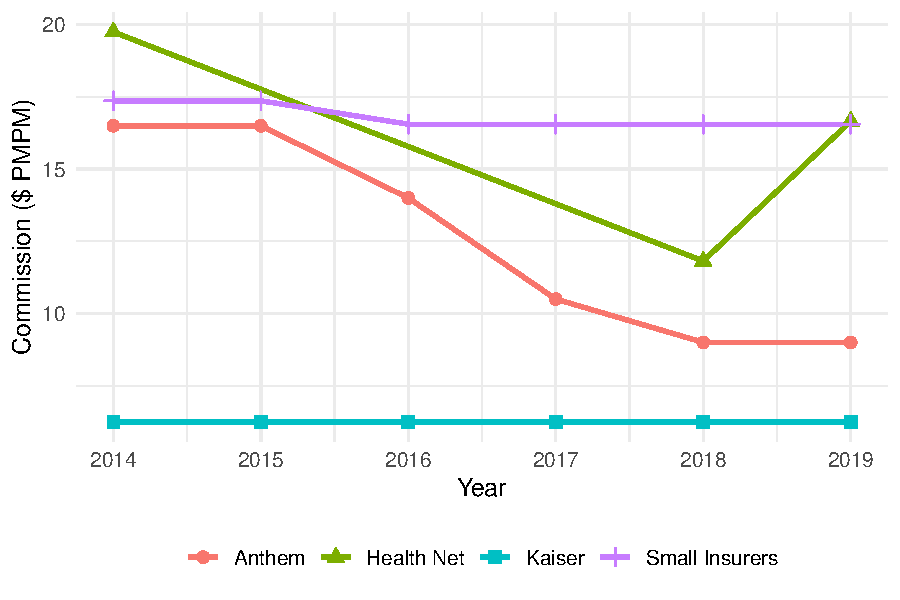
\includegraphics[width=5in]{results/figures/flat_comm.pdf} \\
        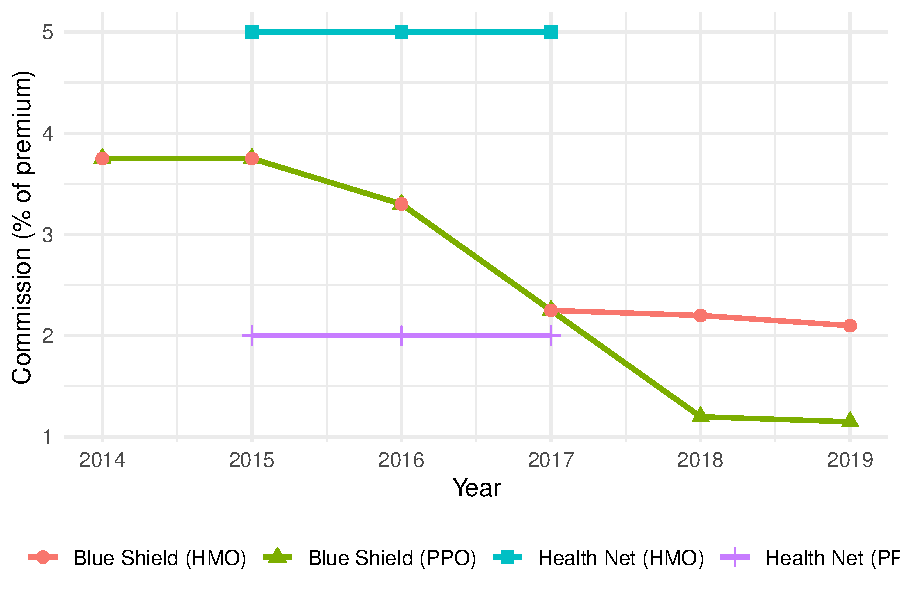
\includegraphics[width=5in]{results/figures/perc_comm.pdf}
    \end{tabular}
}
\label{fig:commissions}
\end{minipage}
\end{figure}

% Which insurer is SH?  Sharp? In the text we use per member per year, so we should be consistent in the figure here

%Global: Let's use "regional insurers" instead of  "small insurers"

% In panel (a), I think it would be better to have the y-axis go down to 0 so it doesn't look like Kaiser pays nothing

\newpage
\begin{figure}[htb]
\centering
\begin{minipage}[h]{6in}
\caption[]{\textbf{Enrollment by Channel, 2014--2019}\footnote{Count of insured households enrolled in a Covered California plan in each year, by assistance channel.}}
\centerline{%
    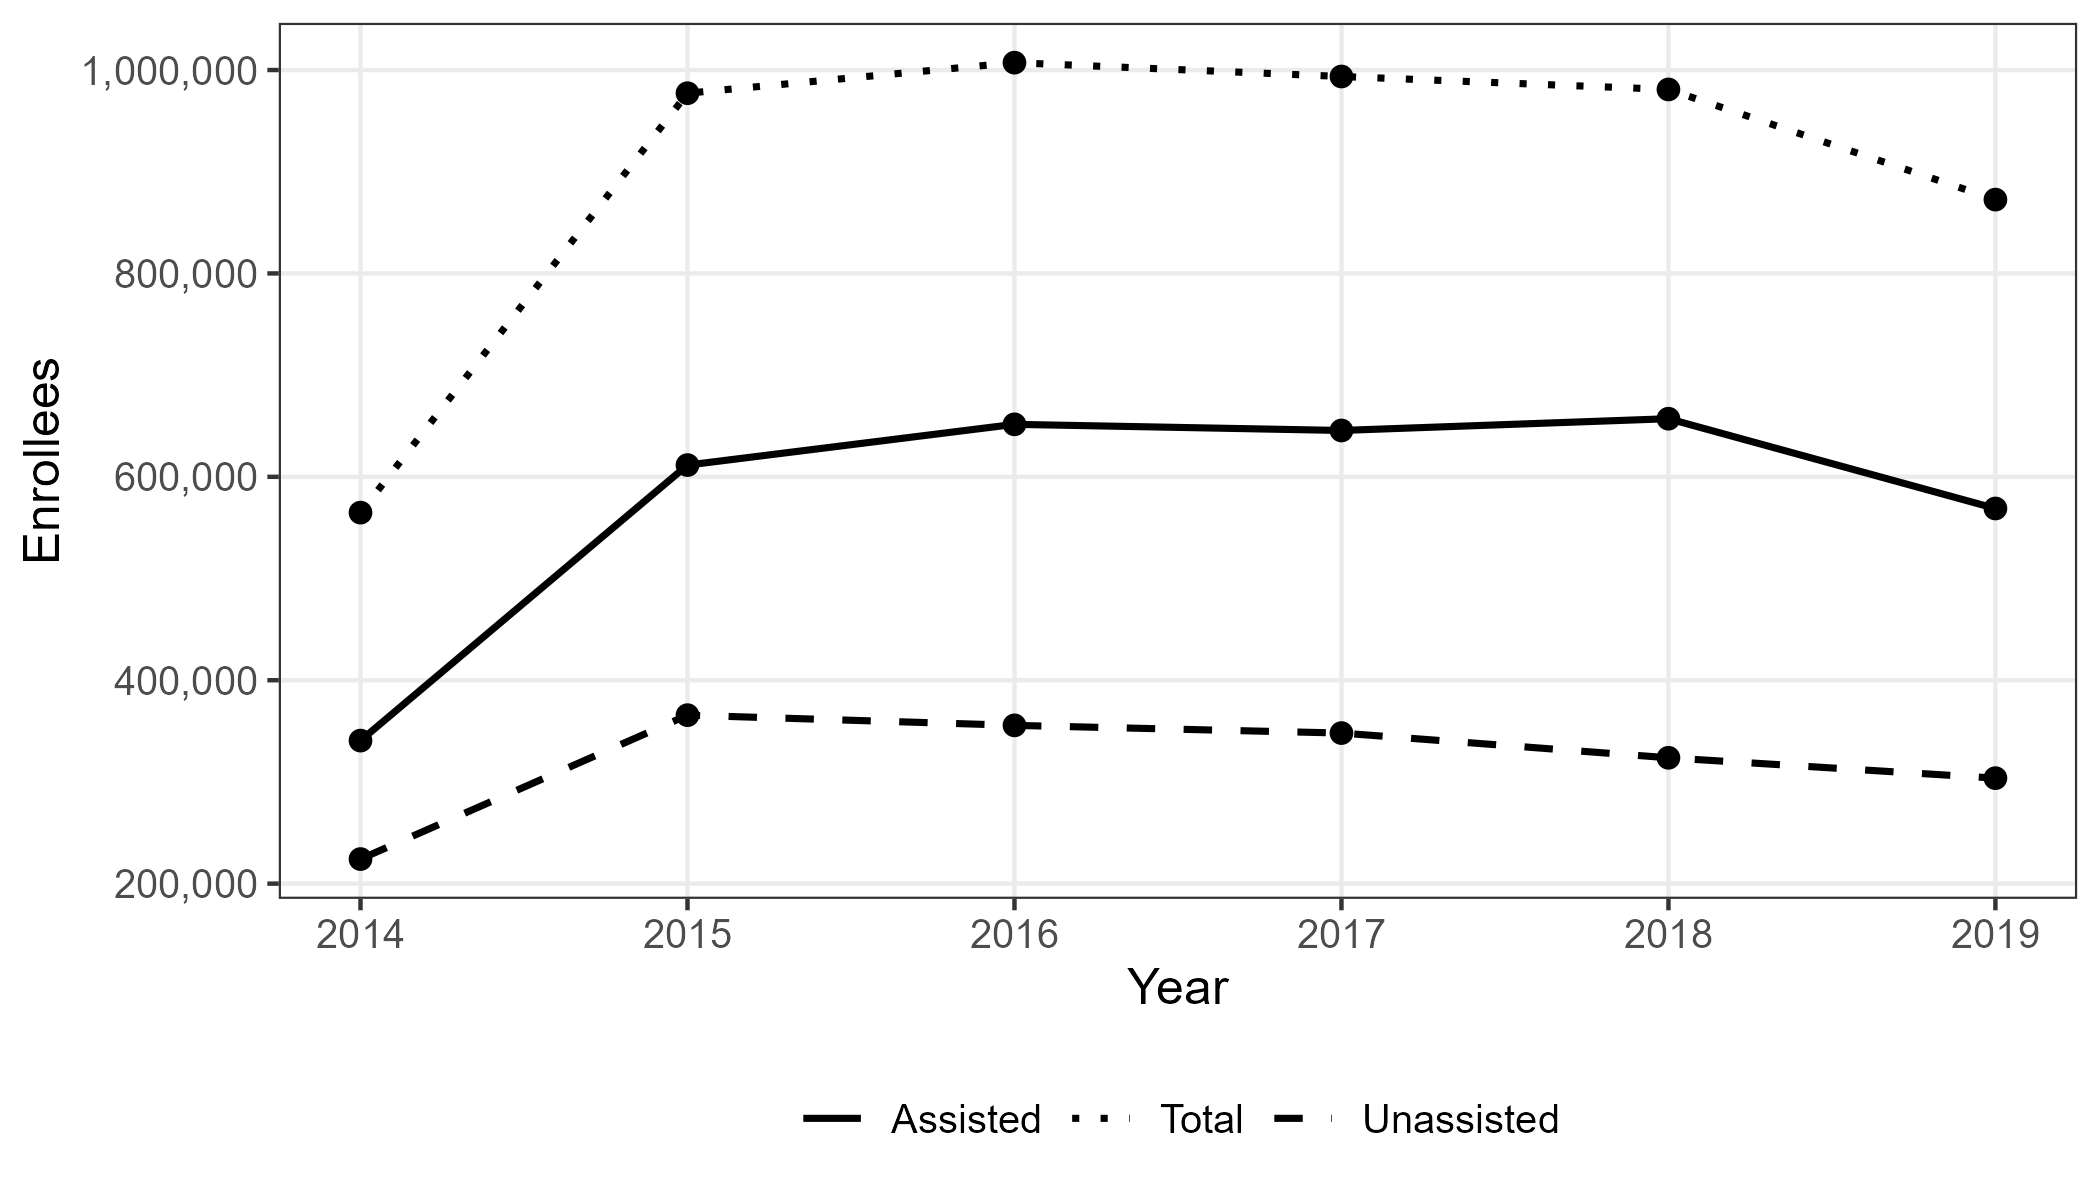
\includegraphics[width=5in]{results/figures/enrollee_count.png}
}
\label{fig:enrollee-count}
\end{minipage}
\end{figure}


\newpage
\begin{figure}[htb]
\centering
\begin{minipage}[h]{6in}
\caption[]{\textbf{Distribution of Propensity Scores for Decision Assistance}\footnote{Propensity scores from a logistic regression of decision assistance on household characteristics, including household income, racial and ethnic composition, age distribution, gender composition, and household size.}}
\centerline{%
    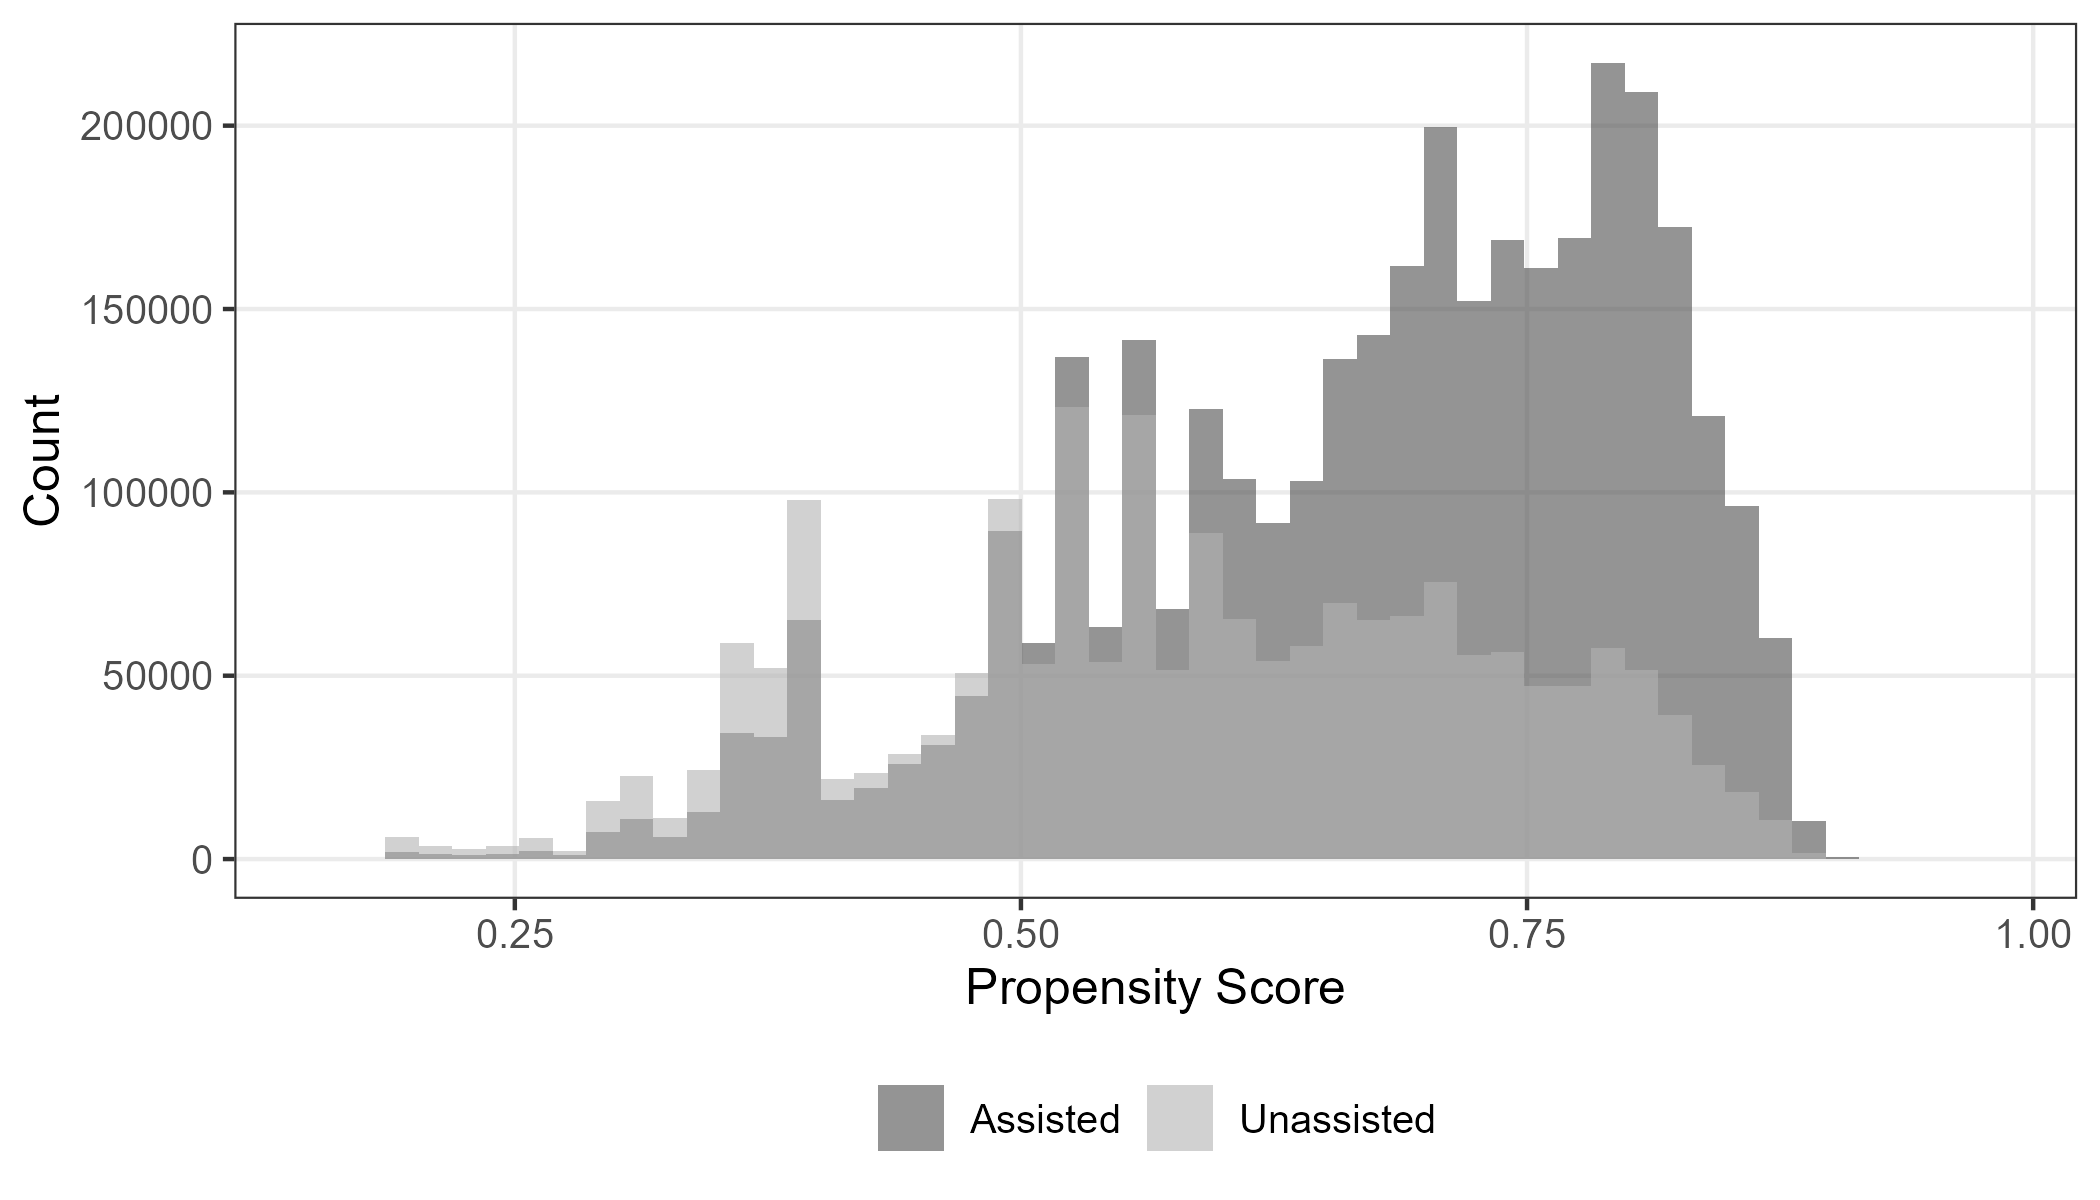
\includegraphics[width=5in]{results/figures/ps_assist_full.png}
}
\label{fig:ps-balance}
\end{minipage}
\end{figure}


\newpage
\begin{figure}[htb]
\centering
\begin{minipage}[h]{6in}
\caption[]{\textbf{Covariate Balance Before and After Inverse-Propensity Weighting}\footnote{Standardized mean differences between assisted and unassisted households. ``Adjusted'' reflects IPW-ATT weights where treated households receive weight 1 and untreated households receive weight $p/(1-p)$, with $p$ denoting the estimated propensity score (see Figure~\ref{fig:ps-balance}).}}
\centerline{%
    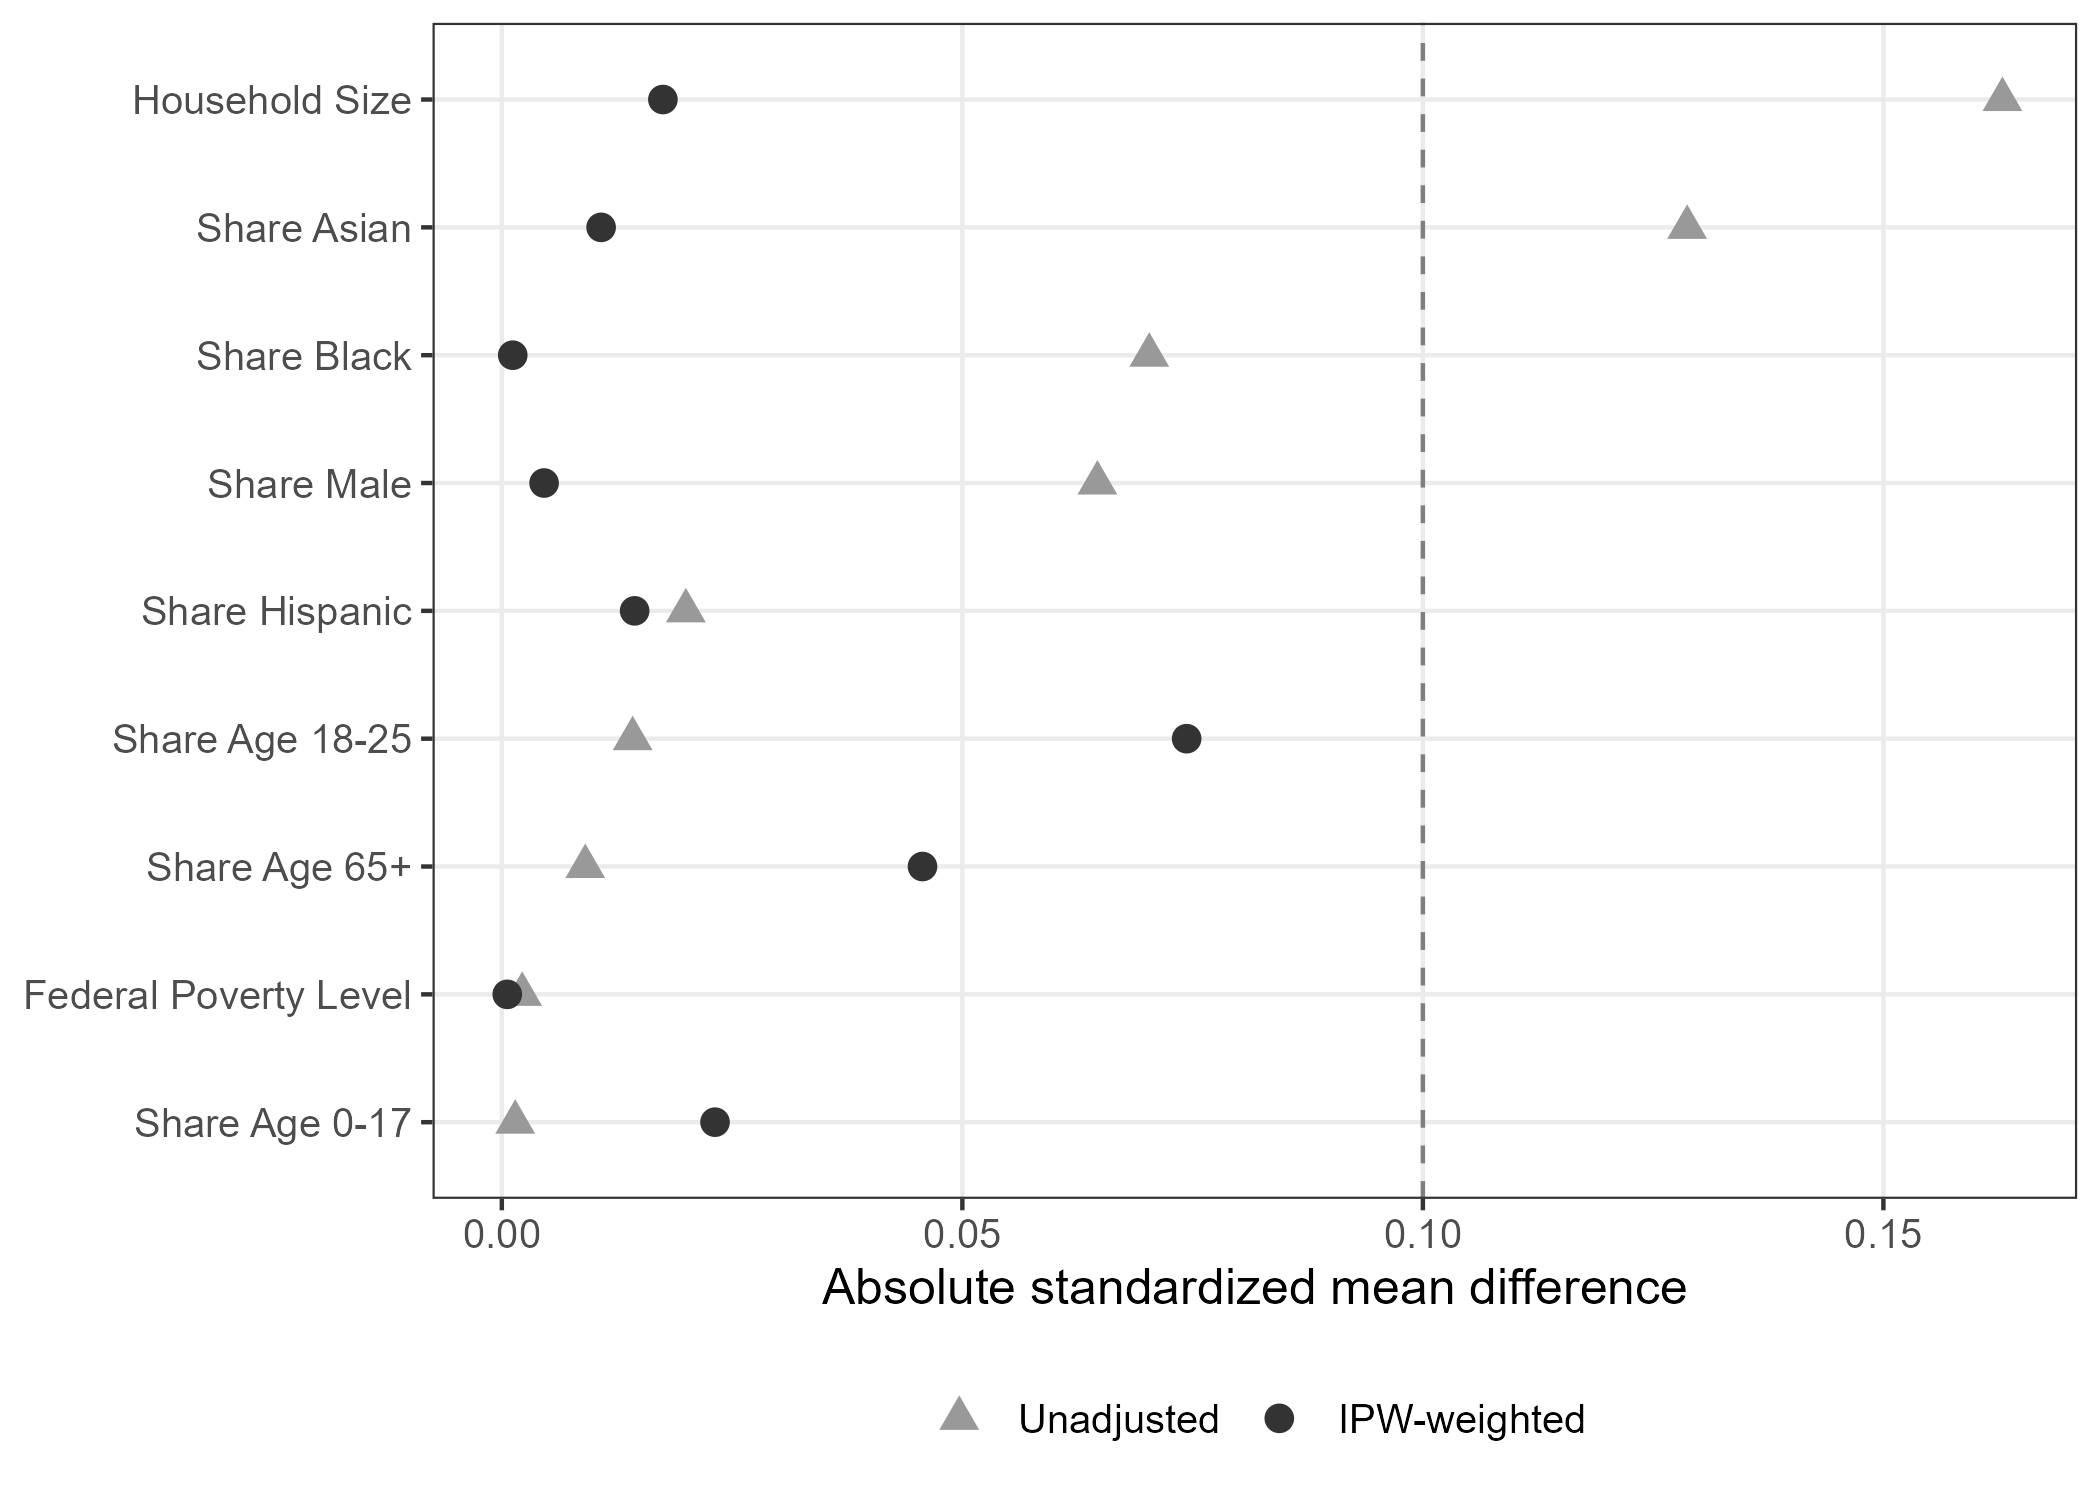
\includegraphics[width=5in]{results/figures/cov_balance.png}
}
\label{fig:cov-balance}
\end{minipage}
\end{figure}


\newpage
\begin{figure}[htb]
\centering
\begin{minipage}[h]{6in}
\caption[]{\textbf{ATT of Decision Assistance on Insurer Choice}\footnote{Estimated ATT as described in Section~\ref{sec:causal}, aggregated to the insurer level. Bars show 95\% confidence intervals from a stratified bootstrap that resamples households within region-year cells.}}
\centerline{%
    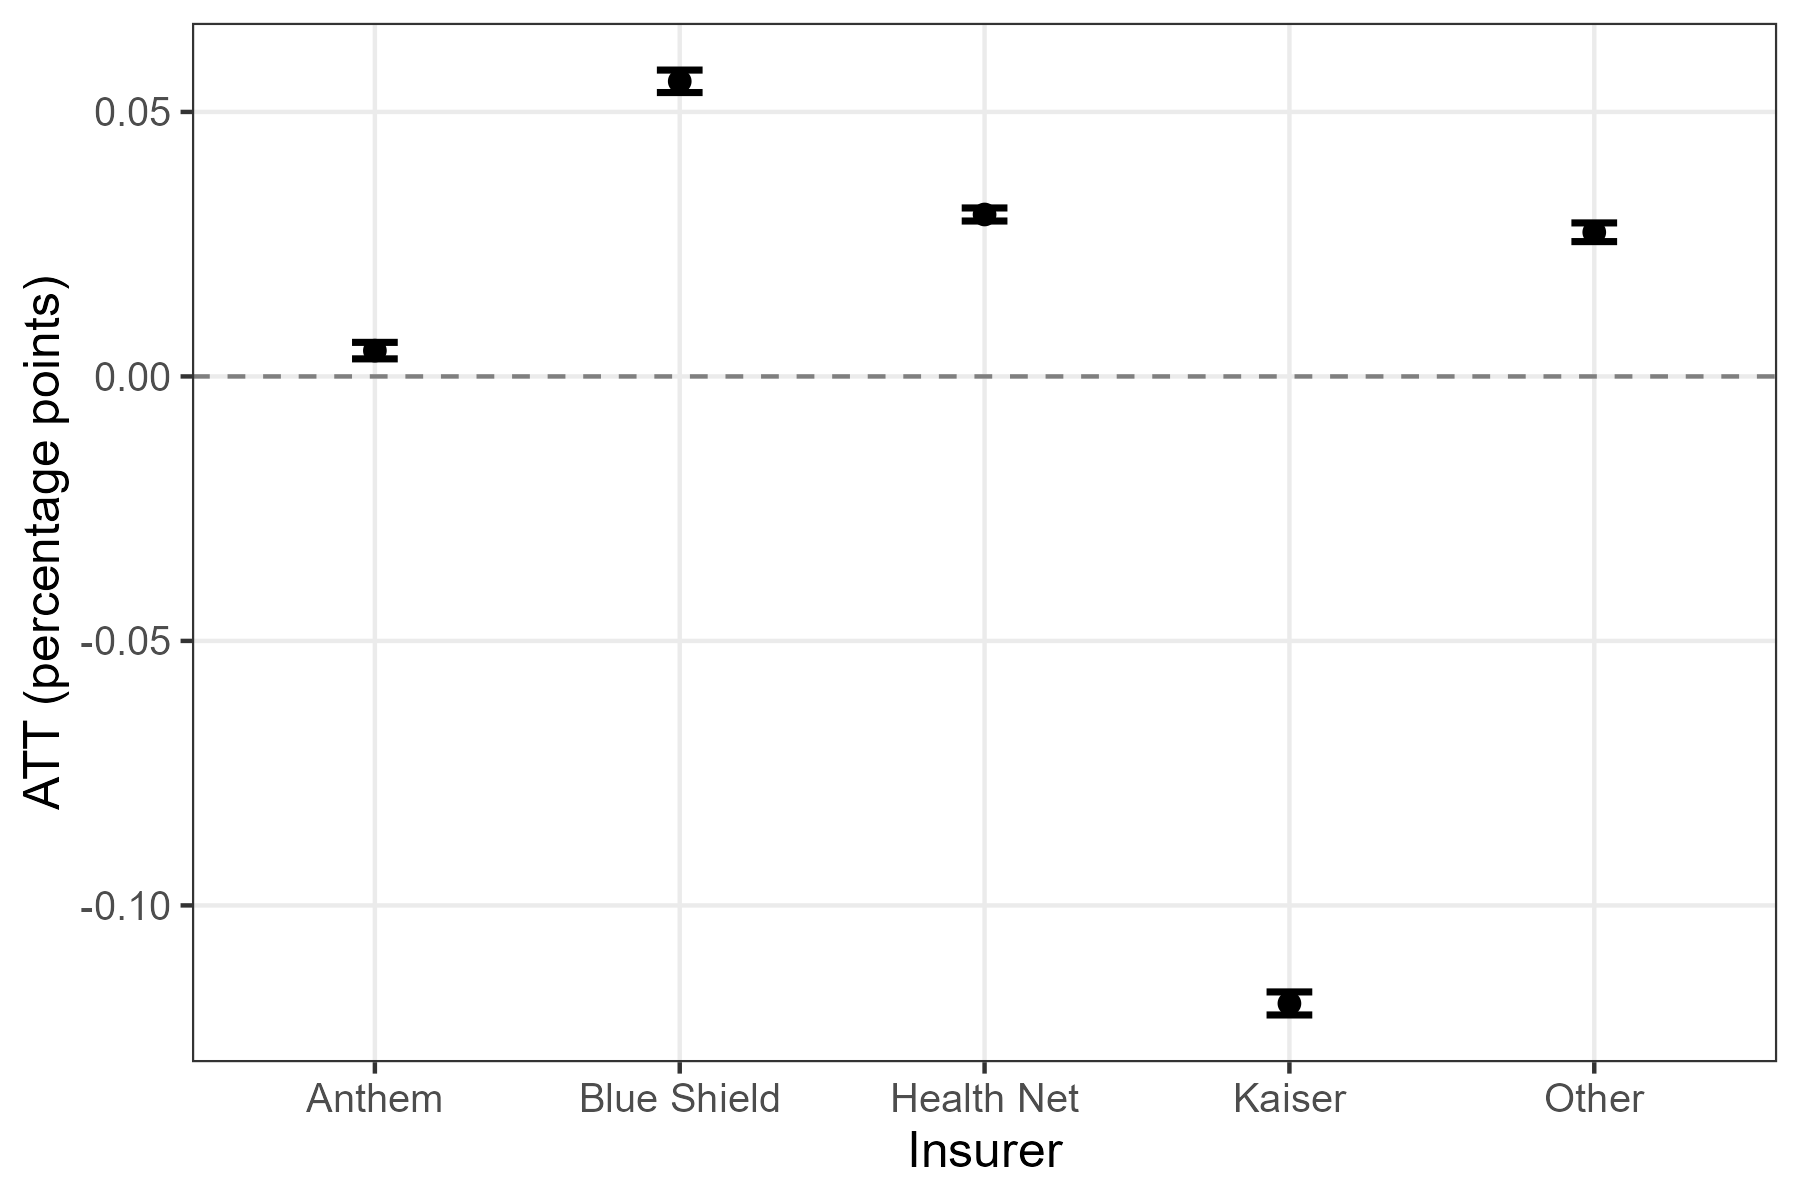
\includegraphics[width=5in]{results/figures/choice_insurer.png}
}
\label{fig:choice-insurer}
\end{minipage}
\end{figure}


\newpage
\begin{figure}[htb]
\centering
\begin{minipage}[h]{6in}
\caption[]{\textbf{ATT of Decision Assistance on Metal Tier Choice}\footnote{Estimated ATT as described in Section~\ref{sec:causal}, aggregated to the level of metal tier. Bars show 95\% confidence intervals from a stratified bootstrap that resamples households within region-year cells.}}
\centerline{%
    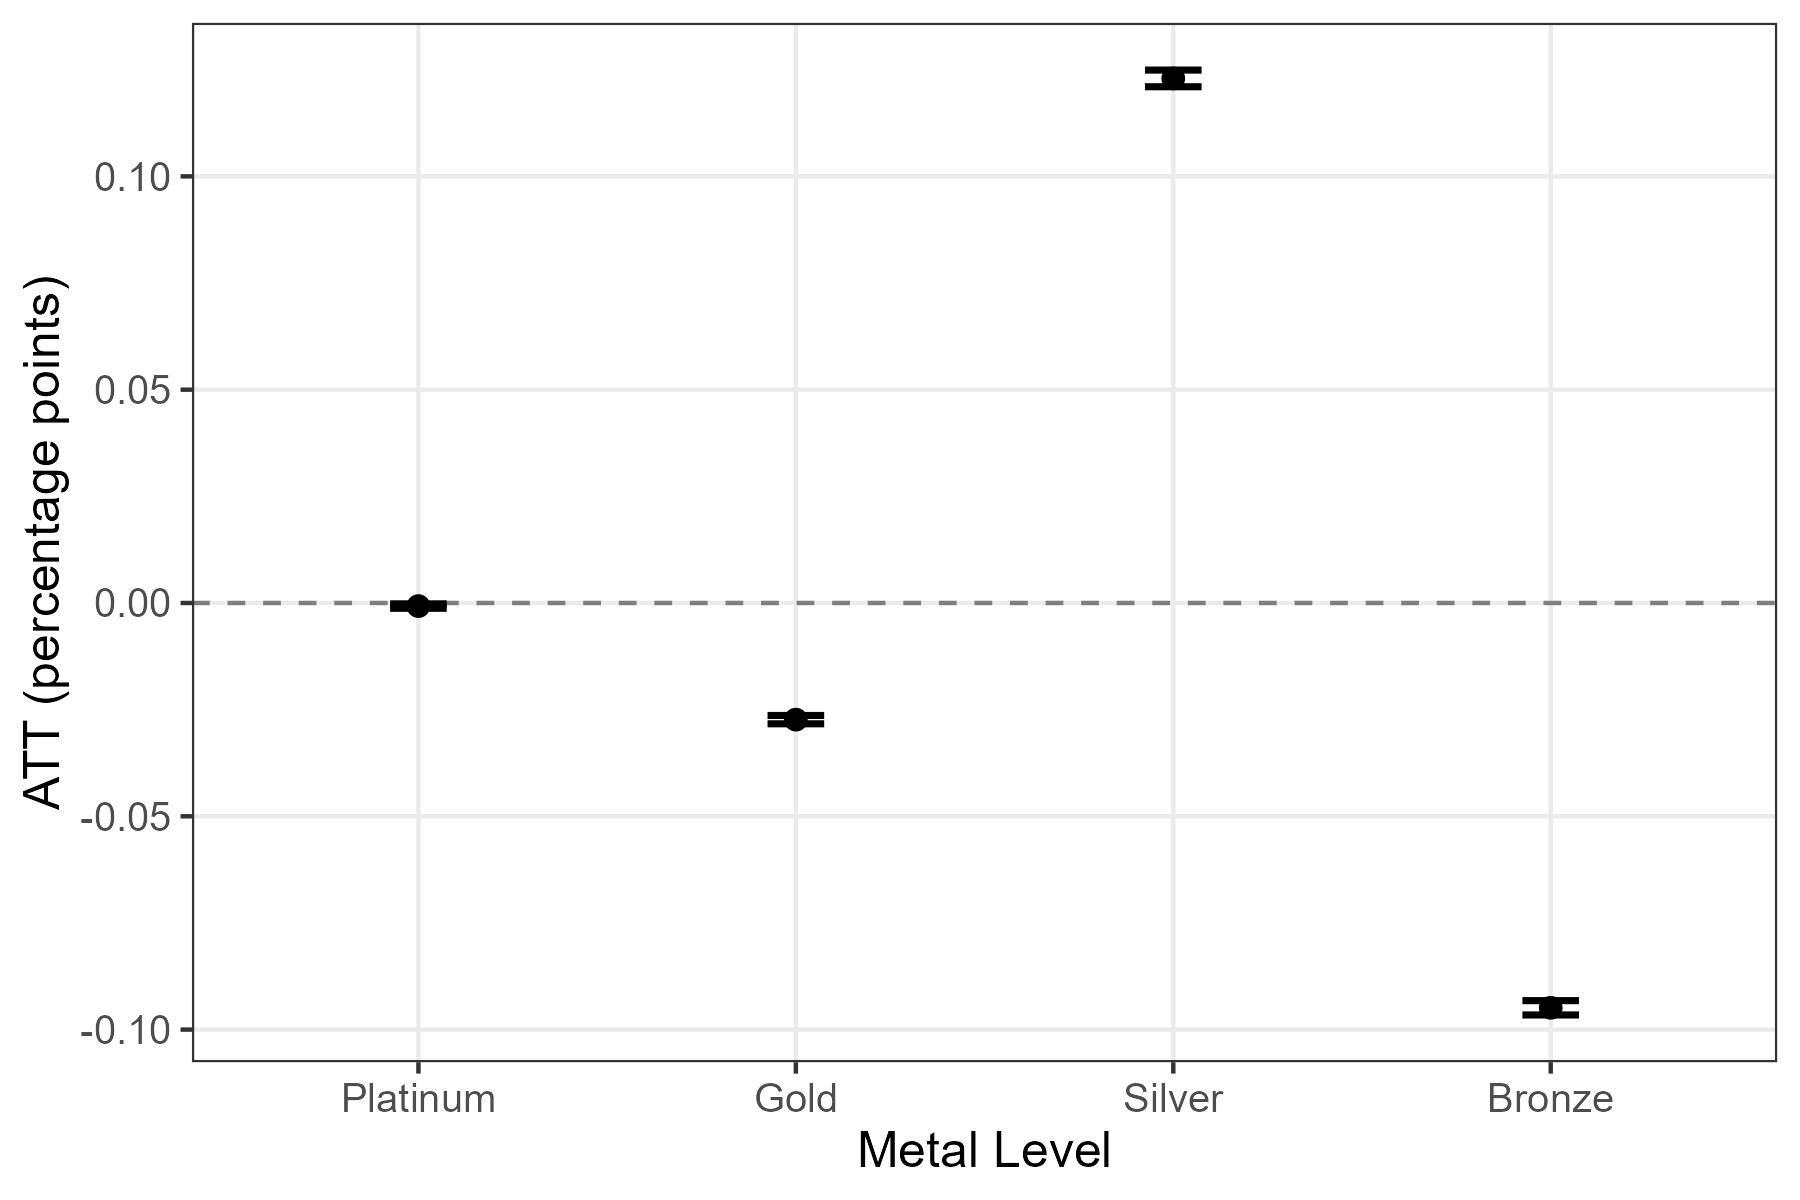
\includegraphics[width=5in]{results/figures/choice_metals.png}
}
\label{fig:choice-metal}
\end{minipage}
\end{figure}


\newpage
\begin{figure}[htb]
\centering
\begin{minipage}[h]{6in}
\caption[]{\textbf{ATT of Decision Assistance on Dominated Choices}\footnote{Estimated ATT as described in Section~\ref{sec:dominated}, on the sample of households with at least one dominated plan in the choice set. Bars show 95\% confidence intervals from a stratified bootstrap that resamples households within region-year cells.}}
\centerline{%
    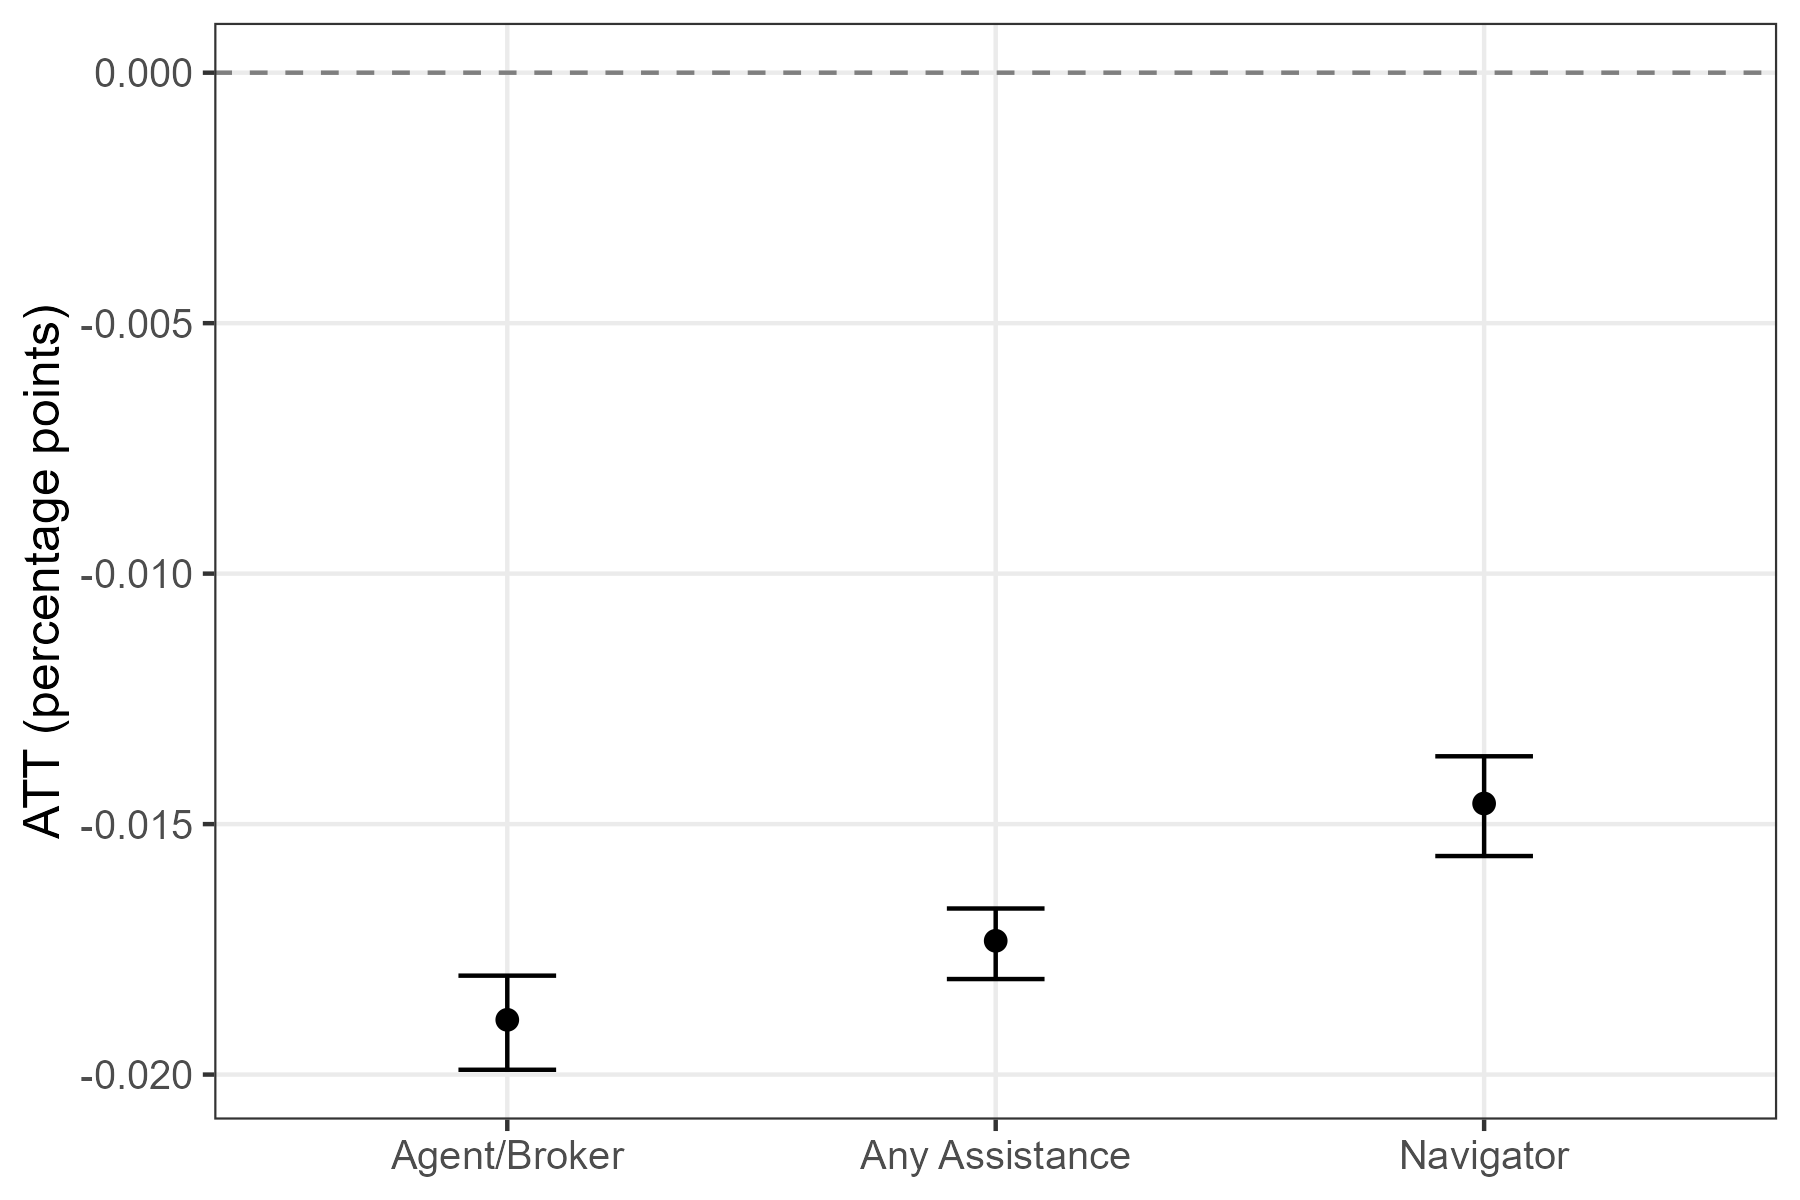
\includegraphics[width=5in]{results/figures/dom_choice.png}
}
\label{fig:dom-choice}
\end{minipage}
\end{figure}


\clearpage
\newpage

\begin{table}
\centering
\footnotesize
\begin{minipage}[h]{6in}
\caption[]{\textbf{Structural Demand Estimates}\footnote{Estimated by maximum likelihood on the pooled sample of all households, weighted by household size, with household-clustered sandwich standard errors. Premiums are net of subsidy and measured in hundreds of dollars. The nesting parameter $\lambda$ governs substitution between exchange plans and the outside option. Navigator $\times$ AV and agent $\times$ AV interactions capture each channel's effect on the valuation of plan generosity. Commission $\times$ agent and its square over 100 capture the effect of per-member-per-month commissions for agent-assisted households. The demographic interactions let price sensitivity, the valuation of generosity, and the value of enrolling vary with household characteristics.}}
\label{tab:demand-estimates}
\renewcommand{\arraystretch}{0.9}
\centerline{%
    \begin{tabular}{lrr}
\hline\hline
Variable & Estimate & Std. Error \\
\hline
Insured (constant) & -3.3870 & 0.0267 \\
Premium & -0.4146 & 0.0031 \\
Actuarial value (AV) & 4.3917 & 0.0283 \\
HMO & -0.2121 & 0.0015 \\
Anthem & 0.3425 & 0.0022 \\
Blue Shield & 0.4556 & 0.0026 \\
Kaiser & 0.5379 & 0.0030 \\
Health Net & 0.2568 & 0.0020 \\
HH size $\times$ premium & -0.0250 & 0.0013 \\
Age 0--17 $\times$ premium & 0.1106 & 0.0095 \\
Age 18--34 $\times$ premium & -0.3785 & 0.0027 \\
Age 35--54 $\times$ premium & -0.1835 & 0.0020 \\
Male $\times$ premium & -0.0176 & 0.0015 \\
Black $\times$ premium & -0.1271 & 0.0048 \\
Hispanic $\times$ premium & -0.2597 & 0.0026 \\
Asian $\times$ premium & -0.1998 & 0.0025 \\
Other race $\times$ premium & -0.0667 & 0.0017 \\
FPL 250--400\% $\times$ premium & 0.3301 & 0.0025 \\
FPL 400+\% $\times$ premium & 0.3647 & 0.0037 \\
HH size $\times$ AV & 0.2419 & 0.0087 \\
Age 0--17 $\times$ AV & -3.6504 & 0.0634 \\
Age 18--34 $\times$ AV & -1.0151 & 0.0161 \\
Age 35--54 $\times$ AV & -0.4380 & 0.0144 \\
Male $\times$ AV & -0.3445 & 0.0117 \\
Black $\times$ AV & 0.5392 & 0.0353 \\
Hispanic $\times$ AV & 0.9899 & 0.0162 \\
Asian $\times$ AV & 0.7227 & 0.0173 \\
Other race $\times$ AV & 0.1667 & 0.0137 \\
FPL 250--400\% $\times$ AV & -3.1298 & 0.0244 \\
FPL 400+\% $\times$ AV & -3.1017 & 0.0371 \\
Enrolled $\times$ HH size & -0.0521 & 0.0070 \\
Enrolled $\times$ share 0--17 & 1.6550 & 0.0431 \\
Enrolled $\times$ share 18--34 & 0.8511 & 0.0134 \\
Enrolled $\times$ share 35--54 & -0.2300 & 0.0117 \\
Enrolled $\times$ share male & 0.1653 & 0.0096 \\
Enrolled $\times$ share Black & -0.6099 & 0.0285 \\
Enrolled $\times$ share Hispanic & -1.3427 & 0.0127 \\
Enrolled $\times$ share Asian & -0.5217 & 0.0142 \\
Enrolled $\times$ share other race & -0.5328 & 0.0112 \\
Enrolled $\times$ FPL 250--400\% & 3.0591 & 0.0188 \\
Enrolled $\times$ FPL $>$400\% & 4.0363 & 0.0278 \\
Navigator $\times$ AV & 1.1850 & 0.0176 \\
Agent $\times$ AV & 0.7291 & 0.0136 \\
Navigator $\times$ premium & -0.0976 & 0.0023 \\
Agent $\times$ premium & -0.0214 & 0.0016 \\
Commission $\times$ agent & 0.0273 & 0.0004 \\
Commission$^2$/100 $\times$ agent & -0.0658 & 0.0011 \\
$\lambda$ (nesting parameter) & 0.3736 & 0.0018 \\
\hline\hline
\end{tabular}

}
\end{minipage}
\end{table}


\newpage
\begin{table}
\centering
\footnotesize
\begin{minipage}[h]{6in}
\caption[]{\textbf{Cost Estimates}\footnote{The risk score equation~\eqref{eqn:risk_score_estimation} is estimated by weighted least squares and held fixed. The claims equation~\eqref{eqn:avg_claims_estimation} is estimated by two-step generalized method of moments jointly with the pricing and commission first-order conditions, with the second-step weight equal to the inverse of the estimated moment covariance. Sandwich standard errors in parentheses. Kaiser silver is the omitted cell in the insurer-by-metal effects. Demographic shares are predicted from the estimated choice model.}}
\label{tab:cost-estimates}
\centerline{%
    \begin{tabular}{lr}
\hline\hline
Variable & Estimate \\
\hline
\emph{Risk score equation} & \\
Constant & 0.3593 \\
 & (0.1680) \\
Share age 0--34 & -0.3029 \\
 & (0.1330) \\
Share male & 0.2096 \\
 & (0.3830) \\
Share family households & 0.9811 \\
 & (0.0876) \\
Share minority & -0.7183 \\
 & (0.0513) \\
Insurer-by-metal effects & Yes \\
\hline
\emph{Claims equation} & \\
Constant & 5.4346 \\
 & (0.0023) \\
Log predicted risk score & 1.3078 \\
 & (0.0063) \\
HMO & -0.2001 \\
 & (0.0182) \\
Year 2015 & 0.0705 \\
 & (0.0069) \\
Year 2016 & 0.2117 \\
 & (0.0073) \\
Year 2017 & 0.2953 \\
 & (0.0084) \\
Year 2018 & 0.4575 \\
 & (0.0092) \\
Anthem & -0.0380 \\
 & (0.0211) \\
Blue Shield & 0.0920 \\
 & (0.0283) \\
Kaiser & 0.5405 \\
 & (0.0406) \\
Health Net & 0.0706 \\
 & (0.0206) \\
Rating-area shares & Yes \\
\hline
\emph{Commission condition} & \\
Cross-market wedge, ANT ($\delta_{f}$) & 0.589 \\
 & (0.107) \\
Cross-market wedge, BS ($\delta_{f}$) & 0.154 \\
 & (0.125) \\
Cross-market wedge, CC ($\delta_{f}$) & -0.632 \\
 & (0.152) \\
Cross-market wedge, HN ($\delta_{f}$) & 0.328 \\
 & (0.117) \\
Cross-market wedge, KA ($\delta_{f}$) & 2.679 \\
 & (0.168) \\
Cross-market wedge, LA ($\delta_{f}$) & -1.394 \\
 & (0.078) \\
Cross-market wedge, MOL ($\delta_{f}$) & -0.859 \\
 & (0.009) \\
Cross-market wedge, OSC ($\delta_{f}$) & 0.254 \\
 & (0.203) \\
Cross-market wedge, SH ($\delta_{f}$) & -0.221 \\
 & (0.044) \\
Cross-market wedge, VAL ($\delta_{f}$) & -0.236 \\
 & (0.668) \\
Cross-market wedge, WEST ($\delta_{f}$) & 0.567 \\
 & (0.305) \\
\hline\hline
\end{tabular}

}
\end{minipage}
\end{table}


\newpage
\begin{table}
\centering
\footnotesize
\begin{minipage}[h]{6in}
\caption[]{\textbf{Supply-Side Results by Metal Tier}\footnote{Each column reports the within-tier median across plan-cells. Premium is the average premium collected per member, the posted age-40 premium scaled by the average age rating of the plan's enrollees. Markup is that premium less MC (Structural). MC (FOC) is the marginal cost implied by the first-order condition inversion. MC (Structural) is the predicted marginal cost from the risk score and claims equations estimated on rate filing data, net of risk adjustment transfers and reinsurance. Lerner index is the markup divided by the premium.}}
\label{tab:supply-results}
\centerline{%
    \begin{tabular}{lrrrrrrr}
\hline\hline
Metal & N & Premium & Markup & MC (FOC) & MC (Structural) & Lerner & Commission \\
\hline
Bronze & 668 & 362.73 & 44.81 & 252.20 & 314.23 & 0.124 & 11.84 \\
Silver & 493 & 484.44 & 116.41 & 406.47 & 350.47 & 0.242 & 14.00 \\
Gold & 531 & 549.00 & 138.87 & 429.88 & 384.44 & 0.255 & 14.00 \\
Platinum & 493 & 617.03 & 143.93 & 418.68 & 422.62 & 0.240 & 15.89 \\
\hline\hline
\end{tabular}

}
\end{minipage}
\end{table}


\newpage
\begin{table}
\centering
\footnotesize
\begin{minipage}[h]{6in}
\caption[]{\textbf{Counterfactual Premium, Coverage, and Welfare Effects}\footnote{Each row reports the change relative to the baseline equilibrium, averaged across region-year cells, for a given counterfactual scenario. $\tau$ is the substitution rate for the zero-commission and navigator-expansion families and is blank where it does not apply. $\Delta$ Premium is the share-weighted change in posted premiums. $\Delta$ Uninsured is the change in the share of households taking the outside option, in percentage points. $\Delta$ CS is the change in Small-Rosen consumer surplus, $\Delta V^{nav}$ is the change in the navigator-rule money metric, and $\Delta V^{obj}$ is the change in the objective money metric at the central uninsured-cost calibration; all are defined in Section~\ref{subsec:welfare_measurement}, and the four dollar figures ($\Delta$ Premium, $\Delta$ CS, $\Delta V^{nav}$, and $\Delta V^{obj}$) are per member per year. The low and high uninsured-cost cases are in Table~\ref{tab:cf-band}.}}
\label{tab:cf-results}
\centerline{%
    \begin{tabular}{llrrrrr}
\hline\hline
Scenario & $\tau$ & $\Delta$ Premium & $\Delta$ Uninsured (pp) & $\Delta$ CS & $\Delta V^{nav}$ & $\Delta V^{obj}$ \\
\hline
Baseline & -- & 0.00 & 0.0 & 0.00 & 0 & 0 \\
Zero commission & 0.00 & 71.41 & 6.1 & -272.38 & -119 & -412 \\
Zero commission & 0.50 & 6.21 & 2.8 & -107.04 & -46 & -183 \\
Zero commission & 1.00 & -54.07 & -0.2 & 127.50 & 30 & 30 \\
Low uniform commission & -- & -6.85 & 0.6 & -4.57 & -14 & -47 \\
Aligned commissions & -- & -0.50 & -0.0 & 5.57 & 22 & 7 \\
Scaled commission (50\%) & -- & 1.79 & 0.7 & -1.55 & -15 & -43 \\
Flat-fee mandate & -- & 2.64 & 0.1 & -1.62 & 1 & -16 \\
Navigator defunding (50\%) & -- & 9.06 & 0.1 & -36.19 & -10 & -12 \\
Agents to navigators (endog.\ commissions) & 0.50 & -21.32 & -0.1 & 53.62 & 10 & 12 \\
\hline\hline
\end{tabular}

}
\end{minipage}
\end{table}


\newpage
\begin{table}
\centering
\footnotesize
\begin{minipage}[h]{6in}
\caption[]{\textbf{Objective Welfare Effect by Uninsured-Cost Calibration}\footnote{Change in the objective money-metric welfare measure relative to the baseline equilibrium, per member per year, under the low, central, and high valuations of the cost of being uninsured described in Section~\ref{subsec:welfare_measurement}. The band reflects the calibration of the cost of being uninsured, principally the mortality valuation; it is distinct from the sampling uncertainty in the estimated parameters. Scenarios are described in Section~\ref{subsec:cf_design}.}}
\label{tab:cf-band}
\centerline{%
    \begin{tabular}{lrrr}
\hline\hline
Scenario & $\Delta V^{obj}$ low & central & high \\
\hline
Baseline & 0 & 0 & 0 \\
Zero commission & & & \\
\quad $\tau=0.00$ & -43 & -412 & -624 \\
\quad $\tau=0.50$ & -12 & -183 & -280 \\
\quad $\tau=1.00$ & 21 & 30 & 35 \\
Low uniform commission & -7 & -47 & -69 \\
Aligned commissions & 9 & 7 & 6 \\
Scaled commission & & & \\
\quad 50\% & -3 & -43 & -66 \\
Flat-fee mandate & -4 & -16 & -22 \\
Navigator defunding & & & \\
\quad 50\% & -7 & -12 & -15 \\
Agents to navigators (endog.\ commissions) & 9 & 12 & 15 \\
\hline\hline
\end{tabular}

}
\end{minipage}
\end{table}


\newpage
\begin{table}
\centering
\footnotesize
\begin{minipage}[h]{6in}
\caption[]{\textbf{Coverage and Welfare Effects with Bootstrap Standard Errors}\footnote{Change in the uninsured share (percentage points) and in the objective money metric at the central uninsured-cost calibration, per member per year, relative to the baseline equilibrium. Standard errors in parentheses are from a parametric bootstrap over the estimated demand parameters and capture the sampling uncertainty in those estimates, distinct from the calibration band across uninsured-cost valuations in Table~\ref{tab:cf-band}. Scenarios are described in Section~\ref{subsec:cf_design}.}}
\label{tab:cf-se}
\centerline{%
    \begin{tabular}{lrr}
\hline\hline
Scenario & $\Delta$ Uninsured (pp) & $\Delta V^{obj}$ \\
\hline
Remove assistance ($\tau$=0) & 6.1 (0.086) & -412 (6.1) \\
Agents to navigators ($\tau$=1) & -0.2 (0.076) & 30 (5.3) \\
Low uniform commission & 0.6 (0.0057) & -47 (0.42) \\
Aligned commissions & -0.0 (0.00067) & 7 (0.05) \\
Flat-fee mandate & 0.1 (0.001) & -16 (0.12) \\
Navigator defunding & 0.1 (0.02) & -12 (1.4) \\
Agents to navigators (endog.\ comm.) & -0.1 (0.038) & 12 (2.6) \\
\hline\hline
\end{tabular}

}
\end{minipage}
\end{table}


\newpage
\begin{table}
\centering
\footnotesize
\begin{minipage}[h]{6in}
\caption[]{\textbf{Producer Surplus and Government Cost by Scenario}\footnote{Change relative to the baseline equilibrium, per member per year, averaged across region-year cells. Producer surplus is the insurer margin, the age-rated premium collected less marginal cost, summed over enrolled members and net of commissions paid to agents less the administrative cost they replace. Subsidies are the advance premium tax credit actually paid, capped at the household premium, on enrolled households. Government cost is subsidies plus cost-sharing reduction payments and uncompensated care, less mandate penalty revenue. Scenarios are described in Section~\ref{subsec:cf_design}.}}
\label{tab:cf-fiscal}
\centerline{%
    \begin{tabular}{llrrrrrr}
\hline\hline
Scenario & $\tau$ & $\Delta$ Producer surplus & $\Delta$ Subsidies & $\Delta$ CSR & $\Delta$ Uncomp.\ care & $\Delta$ Penalties & $\Delta$ Gov.\ cost \\
\hline
Baseline & -- & 0 & 0 & 0 & 0 & 0 & 0 \\
Zero commission & 0.00 & -49 & -193 & -20 & 146 & 32 & -100 \\
Zero commission & 0.50 & -30 & -109 & -9 & 66 & 14 & -66 \\
Zero commission & 1.00 & -27 & -46 & 6 & -6 & -1 & -45 \\
Low uniform commission & -- & -9 & -37 & -1 & 14 & 3 & -27 \\
Aligned commissions & -- & 1 & 3 & 2 & -0 & 0 & 5 \\
Scaled commission (50\%) & -- & -3 & -28 & -1 & 16 & 4 & -17 \\
Flat-fee mandate & -- & 2 & -9 & -0 & 3 & 1 & -7 \\
Navigator defunding (50\%) & -- & 2 & 3 & -1 & 2 & 1 & 4 \\
Agents to navigators (endog.\ commissions) & 0.50 & -11 & -18 & 2 & -3 & -1 & -17 \\
\hline\hline
\end{tabular}

}
\end{minipage}
\end{table}



\newpage
\begin{figure}[htb]
\centering
\begin{minipage}[h]{6in}
\caption[]{\textbf{Marginal Cost Validation}\footnote{FOC-implied marginal cost versus structural prediction from risk score and claims regressions. Each point represents a plan in a region-year cell. The dashed line is the 45-degree line.}}
\centerline{%
    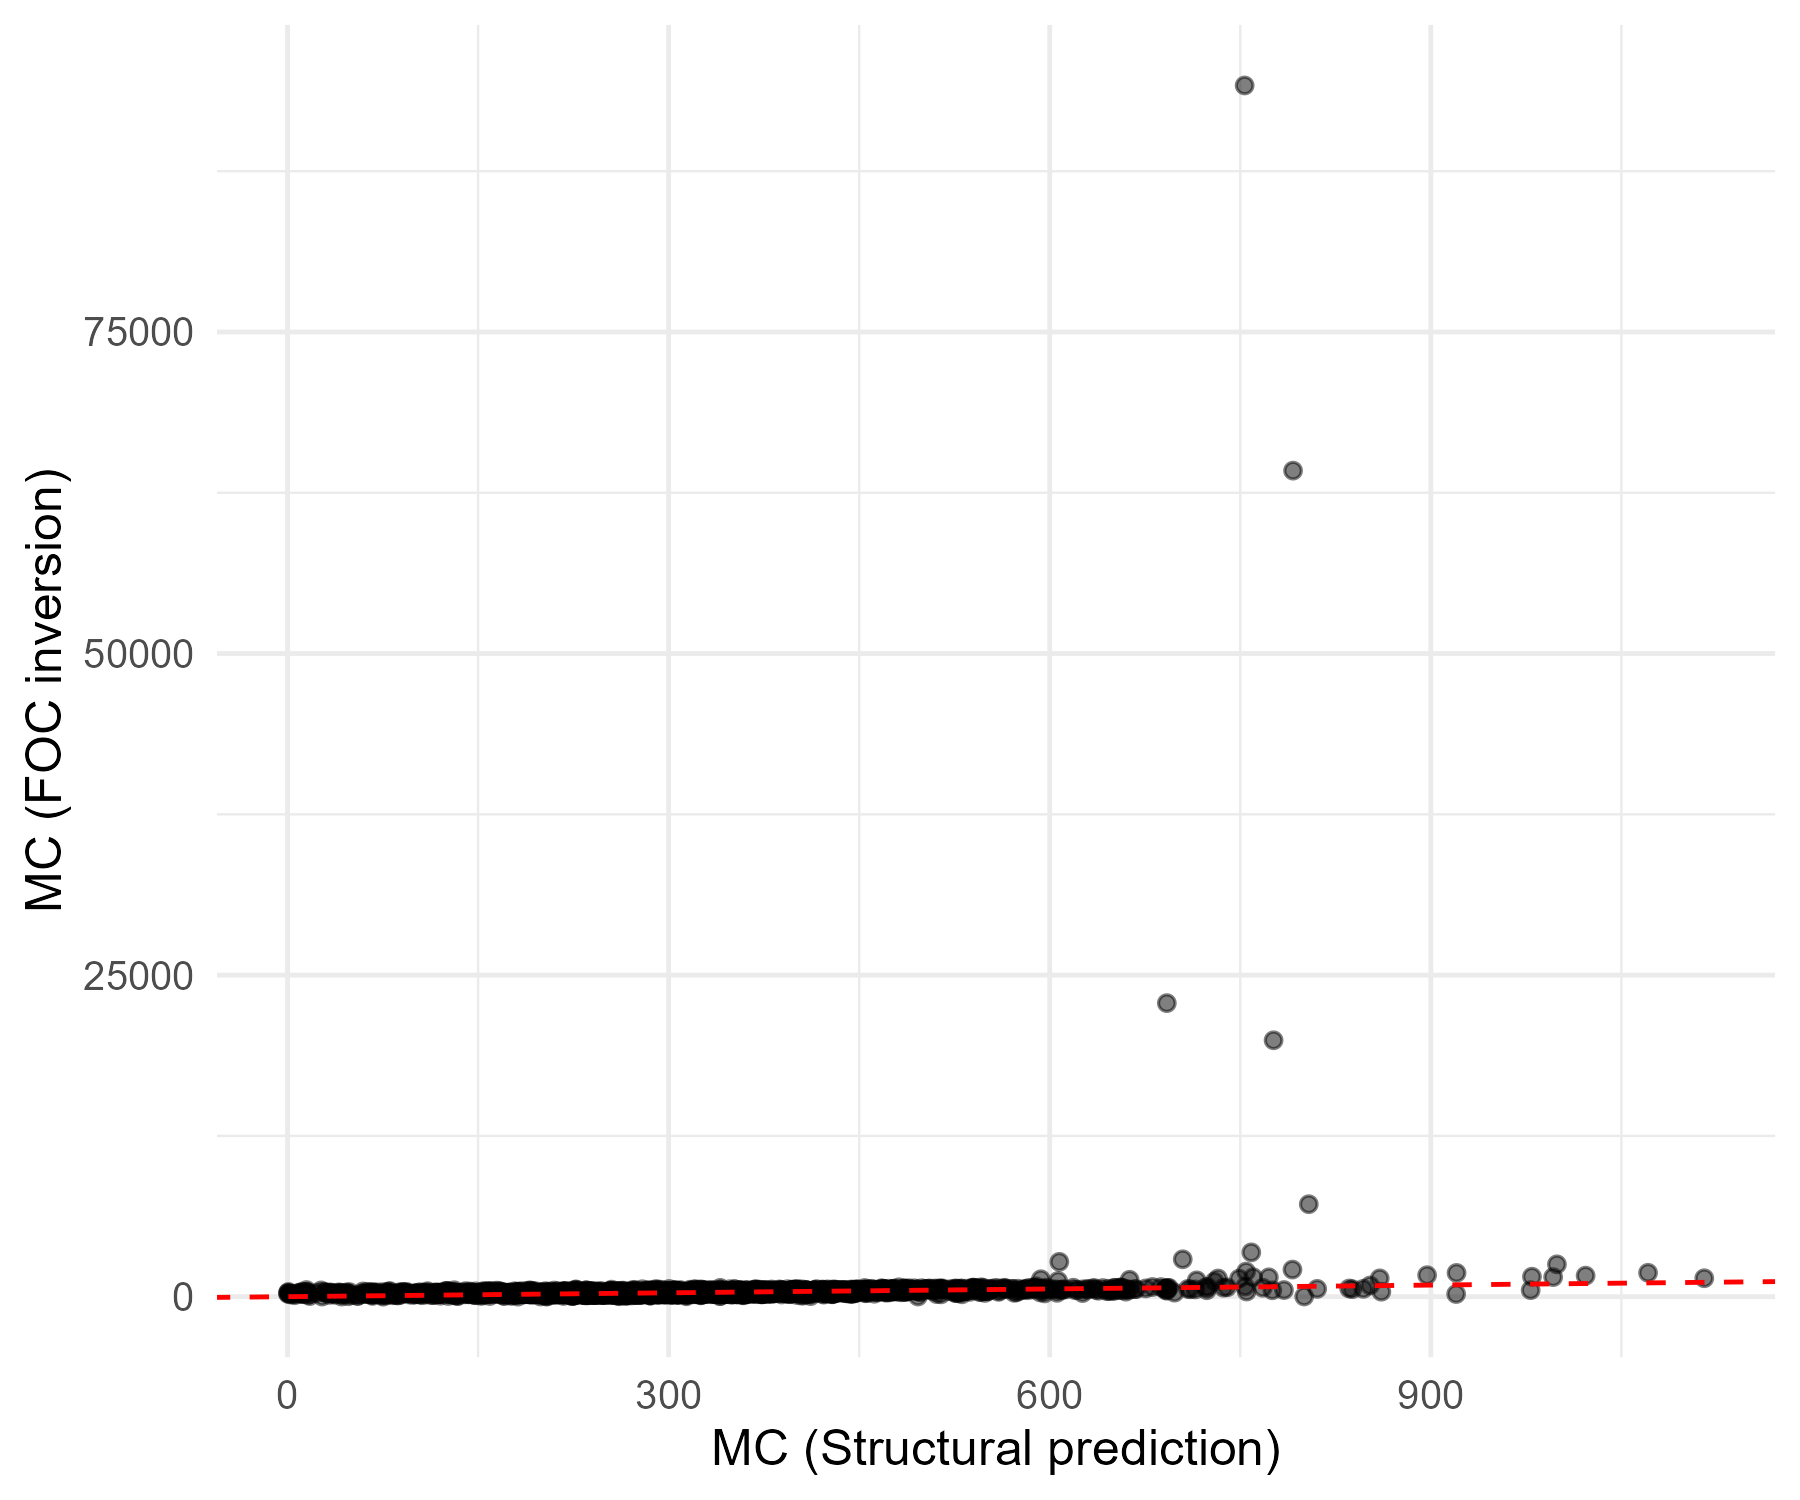
\includegraphics[width=5in]{results/figures/supply_mc_foc_vs_structural.png}
}
\label{fig:mc-validation}
\end{minipage}
\end{figure}


\end{document}


